\documentclass{article}
\usepackage[utf8]{inputenc}
\usepackage{geometry}
\geometry{a4paper, margin=1in}
\usepackage{amsmath, amssymb}
\usepackage{booktabs}
\usepackage{graphicx}
\usepackage{caption}
\usepackage{subcaption}
\usepackage{float}
\usepackage{array}
\usepackage{xcolor}
\usepackage{siunitx}
\usepackage{hyperref}
\usepackage{multirow}


% For line spacing (many journals require 1.5 or double)
\usepackage{setspace}
\doublespacing  % or \onehalfspacing

% For APA-style references (if required)
\usepackage[style=apa,sortcites=true,sorting=nyt,backend=biber]{biblatex}
\addbibresource{references.bib}
% For Times New Roman font
\usepackage{times}

\usepackage{xcolor}
\usepackage{pagecolor}
\usepackage{ifthen}

% Set to 1 for night mode, 0 for day mode
\def\nightmode{1}

\ifthenelse{\equal{\nightmode}{0}}{
    \definecolor{darkbg}{RGB}{30,30,30}
    \pagecolor{darkbg}
    \color{white}
    \hypersetup{colorlinks=true, linkcolor=cyan, urlcolor=cyan}
}{
    \pagecolor{white}
    \color{black}
}



% Table formatting
\newcolumntype{L}[1]{>{\raggedright\arraybackslash}p{#1}}
\newcolumntype{C}[1]{>{\centering\arraybackslash}p{#1}}
\newcolumntype{R}[1]{>{\raggedleft\arraybackslash}p{#1}}

\begin{document}

\title{Doing More with Less: How Cultural Personas Bridge the Cost-Performance Gap in LLMs}
\author{Youssef Hariri \\ yousef.hariri@rennes-sb.com}
\date{September 25, 2026 (revised)}
\maketitle


\begin{abstract}

Cultural personas have emerged as a promising technique for enhancing creativity in Large Language Models, yet their effectiveness across different architectures, domains, and economic contexts remains poorly understood. This study provides a systematic evaluation of three cultural personas—Culture\_5 (innovator), Culture\_Expert (implementer), and Culture\_11 (cultural specialist)—across seven large language models representing both Western (Claude, Gemini, GPT, Llama, Mistral) and Eastern (DeepSeek, Qwen) training regions. (Gemini's unique response format, containing reasoning traces not present in other models, limited direct comparability; results are reported for completeness.) Using 100 problems spanning four domains (Creative, General Knowledge, Instruction, Reasoning), we analyze 31,605 judge ratings of 3,516 model responses using a multi-judge evaluation framework, treating the response (the mean of its nine judge ratings) as the unit of analysis.

Inter-rater reliability over the full dataset was fair-to-moderate for all four core creativity dimensions (Fleiss' \(\kappa = 0.31\)--\(0.33\)); we focus on Novelty as the construct central to our research question. Persona effectiveness follows a contingency model rather than a universal rule: effects are highly model-dependent. Claude with Culture\_5 showed a large positive effect on Novelty (\(d = 1.087\)), while Qwen with Culture\_11 showed a medium negative effect (\(d = -0.638\)); 11 of 21 model-persona comparisons reached statistical significance. Domain-specific analysis revealed that Culture\_5 performed best on General Knowledge (\(d = 0.628\)) and Reasoning (\(d = 0.545\)), while Culture\_11 harmed Novelty across all domains (\(d = -0.149\) to \(-0.229\)).

Economically, six model-persona combinations achieved significant performance gains at equal or lower cost than their large baselines (40-87\% savings for GPT and Claude; cost parity for DeepSeek). The Efficiency Gain Ratio (EGR) provides a unified metric: GPT combinations achieved exceptional economic value (EGR up to 9.15, where EGR > 5 indicates exceptional value). Training region did not moderate persona effects (interaction \(p = 0.445\); Bayes Factor \(= 0.331\)), suggesting training origin is less important than architectural factors.

These findings demonstrate that persona effectiveness is contingent on model architecture and task domain, and establish the economic viability of small models with personas for novelty generation. For practitioners, the path forward is not to seek a single "best" persona, but to match the right persona to the right model for the right task.

\textbf{Keywords:} Large Language Models, Cultural Personas, Novelty, Cross-Architecture Evaluation, Cost-Performance Analysis
\end{abstract}

\noindent\textbf{DOI:} 10.5281/zenodo.19533619
\section*{List of Abbreviations}

\begin{center}
\begin{tabular}{ll}
\textbf{Abbreviation} & \textbf{Definition} \\
EGR & Efficiency Gain Ratio \\
LLM & Large Language Model \\
MoE & Mixture-of-Experts \\
PBP & Persona-Based Prompting \\
RLHF & Reinforcement Learning from Human Feedback \\
SFT & Supervised Fine-Tuning \\
SLM & Small Language Model \\
\end{tabular}
\end{center}

\section{Introduction}

Large Language Models have demonstrated remarkable capabilities across diverse domains, yet their ability to generate truly creative outputs remains contested. While LLMs excel at producing fluent and coherent text, research reveals a "creativity gap": they surpass average human performance in divergent association tasks but consistently fail to match highly creative human individuals (\cite{ antoine_bellemare_pepin_a5621579, vikram_arora_67282d96}). This gap is further complicated by the "Alignment Tax"—the homogenization of outputs resulting from Reinforcement Learning from Human Feedback, which suppresses creative diversity in favor of safe, predictable responses (\cite{ behnam_mohammadi_78154429,michael_ryan_c7257c47}).

One promising approach to unlocking suppressed creativity is persona-based prompting (PBP). By embedding descriptive social roles into system prompts, PBP aims to overcome the model's default "helpful assistant" persona and tap into its latent ability to simulate diverse cognitive styles (\cite{christina_lu_520bd0ae,jing_yang_699d9c2c}). Prior work has demonstrated that personas can shift model judgment by 10-15\% and improve Theory-of-Mind reasoning (\cite{tiancheng_hu_49571f40,gerard_yeo_2544df62}). However, recent benchmarks reveal a performance dissociation: state-of-the-art models sometimes fail to outperform less advanced models in maintaining persona faithfulness, suggesting that persona capability is a distinct dimension of intelligence that does not scale linearly with model size (\cite{vinay_samuel_301ec4c0}).

Despite these advances, critical gaps remain. First, existing evaluations have primarily focused on Western models, leaving open the question of how personas interact with models trained on Eastern cultural corpora. The "Cultural Gene" hypothesis posits that foundational values embedded during pre-training remain resilient after fine-tuning (\cite{emanuel_z__fenech_borg_a4a3e300}), but empirical evidence across diverse architectures is lacking. Second, domain-specific effects of personas remain underexplored. While the "Cultural Persona Paradox" suggests that personas intended to increase sensitivity can instead activate stereotypical noise (\cite{mahammed_kamruzzaman_a0ec385e, kharchenkoHowWellLLMs2024}), it is unclear which domains are most vulnerable to this effect. Third, the economic implications of persona-based steering have received little attention. With inference costs accounting for up to 90\% of production expenses (\cite{francisco_dur_n_a28bb68b}), understanding whether small models with personas can achieve comparable performance to large models at lower cost is critical for both sustainability and accessibility (\cite{anuj_kumar_1c38e9e4, jennifer_haase_36a334aa}).

This study addresses these gaps through a systematic evaluation of seven large language models—representing both Western (Claude, Gemini, GPT, Llama, Mistral) and Eastern (DeepSeek, Qwen) training regions—across 100 problems spanning four domains: Creative, General Knowledge, Instruction, and Reasoning. We evaluate three cultural personas designed along creativity dimensions: Culture\_5 (innovator), Culture\_Expert (implementer), and Culture\_11 (cultural specialist). Our analysis integrates multiple methodological approaches: inter-rater reliability assessment to validate judge consistency, effect size estimation with bootstrap confidence intervals, two-way ANOVA for interaction effects, and economic metrics including the Efficiency Gain Ratio (EGR).

This study makes five contributions. First, we provide a cross-architecture evaluation of cultural personas across both Western and Eastern models, revealing that persona effectiveness follows a contingency model rather than a universal rule. Second, we identify domain-specific patterns showing that persona effects vary by task type, with Culture\_5 performing best on General Knowledge and Reasoning problems. Third, we demonstrate that inter-rater reliability is fair-to-moderate and statistically indistinguishable across the four core creativity dimensions (\(\kappa = 0.31\)--\(0.33\)) when computed over the full dataset, motivating a theory-driven focus on Novelty with the remaining dimensions reported as exploratory. Fourth, we introduce the Efficiency Gain Ratio (EGR) as a unified metric for cost-performance evaluation, demonstrating that small models with personas achieve significant performance gains at equal or lower cost than their large baselines (40-87\% savings for GPT and Claude; cost parity for DeepSeek), with GPT combinations achieving exceptional economic value (EGR up to 9.15). Fifth, cross-model comparisons showed that DeepSeek with Culture\_5 achieved comparable Novelty performance to Claude Opus at 60× lower cost, challenging assumptions that only large, expensive models deliver high value responses.

The remainder of this paper is structured as follows. Section 2 reviews related literature on creativity in LLMs, cultural dimensions, persona-based prompting, and cost-performance analysis. Section 3 describes our methodology, including models, personas, problem dataset, evaluation framework, and statistical analyses. Section 4 presents our results, focusing on Novelty as the primary outcome measure. Section 5 discusses the theoretical and practical implications of our findings, situates them within existing literature, and acknowledges limitations. Section 6 concludes with a summary of contributions and directions for future research.

\section{Literature Review}

This review synthesizes three distinct but interconnected streams of research: creativity in Large Language Models, cultural dimensions in AI, and persona-based steering. We then integrate these streams to articulate a contingency model of persona effectiveness and identify the research gaps that motivate this study.

\subsection{Creativity in LLMs}

\subsubsection{The Divergent-Convergent Dichotomy}

The intersection of artificial intelligence and cognitive psychology has necessitated a shift from purely functional evaluations of LLMs to more nuanced psychometric assessments. Central to this shift is the application of Guilford's Structure of Intellect Model, which distinguishes between divergent thinking—the generation of novel and diverse ideas—and convergent thinking—the refinement of ideas into a single, coherent solution (\cite{vikram_arora_67282d96, harsh_kumar_84fce084}). These two modes map directly to the creativity dimensions used in this study: Novelty and Flexibility align with divergent thinking, while Usefulness and Elaboration align with convergent thinking.

Empirical evidence suggests that LLMs exhibit a "creativity gap" when compared to human experts. While state-of-the-art LLMs often surpass average human performance in divergent association tasks, they consistently fail to reach the performance levels of highly creative human individuals (\cite{antoine_bellemare_pepin_a5621579}). This performance is further bifurcated by the creative phase: LLMs excel in divergent phases but struggle in convergent phases requiring selective precision (\cite{harsh_kumar_84fce084}). Following Boden's theory, LLMs primarily demonstrate P-creativity (psychological creativity) rather than H-creativity (historical creativity), as their outputs are fundamentally recombinations of existing training data (\cite{vikram_arora_67282d96, harsh_kumar_84fce084}).

\subsubsection{The Alignment-Creativity Trade-off}

A critical theoretical tension exists between model safety (alignment) and creative potential. Reinforcement Learning from Human Feedback (RLHF), while essential for stabilizing the "helpful assistant" persona, has been found to cause homogenization, reducing semantic entropy and creative diversity (\cite{antoine_bellemare_pepin_a5621579, behnam_mohammadi_78154429}). This "Alignment Tax" results in models that are more predictable but significantly less novel (\cite{michael_ryan_c7257c47}). Research suggests that persona steering may be necessary to "unlock" suppressed creative diversity (\cite{mete_ismayilzada_d0dea915}).

\subsection{Cultural Dimensions in AI}

\subsubsection{Hofstede's and Hall's Frameworks and the "Cultural Gene"}

The evaluation of cultural alignment in LLMs has evolved toward the systematic mapping of models onto established socio-psychological frameworks. The most prominent are Hofstede's Cultural Dimensions Theory and Hall's Cultural Dimensions (high-context vs. low-context communication) (\cite{kharchenkoHowWellLLMs2024, reem_i__masoud_f9cde5f1}). This study integrates both Hofstede's and Hall's frameworks to define the creativity criteria used to design the three cultural personas, following the methodology established in prior work (\cite{haririLLMCreativityMeasuringExplaining2025}).

Research identifies a pervasive "Western-centric" bias in global models like GPT-4, which consistently score high on Individualism and low on Power Distance—values that mirror the demographic profile of their training data (\cite{emanuel_z__fenech_borg_a4a3e300, nicholas_sukiennik_6b60add4}). This "Cultural Gene" of the model—a foundational value set embedded during pre-training—remains resilient even after fine-tuning (\cite{emanuel_z__fenech_borg_a4a3e300}). While Western models favor Individualism and low-context communication, models trained on Eastern corpora exhibit significantly higher scores in Collectivism, Uncertainty Avoidance, and high-context communication styles (\cite{minsang_kim_43ca3c83}).

\subsubsection{The Alignment-Culture Gap}

Alignment processes—Supervised Fine-Tuning (SFT) and RLHF—act as secondary filters that often enforce homogenized value sets (\cite{minsang_kim_43ca3c83}). RLHF tends to pull models toward a "global average" disproportionately influenced by Western liberal values, creating an "Alignment-Culture Gap" where responses lack deep contextual nuance for non-Western contexts (\cite{nicholas_sukiennik_6b60add4}). This underscores the need for cross-architecture evaluation of cultural persona effectiveness.

\subsection{Persona-Based Steering}

\subsubsection{The "Assistant Axis" and Default Personas}

Current LLMs are predominantly aligned to a "helpful assistant" default persona (\cite{christina_lu_520bd0ae}). However, research shows this default can be restrictive; assigning a generic persona does not consistently improve performance compared to a null prompt (\cite{mingqian_zheng_2dd4a908}). Persona-based prompting (PBP) is therefore used to break this axis and elicit specialized reasoning that the default persona might suppress.

\subsubsection{The Persona Effect}

Frameworks like PHAnToM have demonstrated that assigning specific personas significantly affects a model's Theory-of-Mind capabilities (\cite{gerard_yeo_2544df62}). Studies show that when prompted with a detailed social persona, models improve their ability to navigate complex social scenarios, though gains are architecture-dependent (\cite{jing_yang_699d9c2c}). The "Persona Effect" can shift model judgment by 10-15\%, even on tasks where the persona is technically irrelevant (\cite{tiancheng_hu_49571f40}). As persona profiles become more detailed, model responses become more internally consistent (\cite{yuqing_bai_9d1d72ff}).

\subsubsection{Persona Capability as a Distinct Dimension}

Benchmarks like PersonaGym reveal a performance dissociation: state-of-the-art models like GPT-4 sometimes fail to outperform less advanced models in maintaining persona faithfulness (\cite{vinay_samuel_301ec4c0}). This suggests "persona capability" is a distinct dimension of intelligence that does not scale linearly with model size (\cite{vinay_samuel_301ec4c0}). Persona fidelity also fluctuates by task type and social desirability. Models maintain higher fidelity in structured tasks compared to open-ended generation (\cite{jisu_shin_0a44d92a}). This drop is most pronounced when models are assigned traits not socially preferred, suggesting RLHF implicitly guides models toward socially acceptable personas (\cite{manon_reusens_1659b7a7}).

\subsubsection{Research Gaps}

Despite these advances, critical gaps remain. First, existing evaluations have primarily focused on Western models, leaving open how personas interact with Eastern-trained models. Second, domain-specific effects of personas remain underexplored. Third, the economic implications of persona-based steering have received little attention. This study addresses these gaps through a systematic evaluation of seven large language models representing both Western and Eastern training regions across 100 problems spanning four domains.

\subsection{Cost-Performance Analysis}

\subsubsection{The Economic Case for Smaller Models}

The rapid scaling of LLMs has introduced a fundamental tension between performance and escalating costs. Inference accounts for up to 90\% of production costs (\cite{francisco_dur_n_a28bb68b}), leading to "LLM Right-sizing"—determining when smaller, locally deployed models are "good enough" for specific tasks (\cite{jennifer_haase_36a334aa}). Fine-tuned Small Language Models (SLMs) can maintain comparable performance to LLMs while producing significantly lower emissions (\cite{anandita_garg_c5aff6a3,anuj_kumar_1c38e9e4}).

\subsubsection{Efficiency Metrics}

Novel efficiency metrics have been proposed to address real-world deployment constraints. The Carbon Efficient Gain Index (CEGI) quantifies carbon emission per unit of percentage gain per million parameters (\cite{anuj_kumar_1c38e9e4}). The Efficiency Gain Ratio (EGR) unifies performance and cost considerations:

\begin{equation}
EGR = \frac{\text{Performance}_{\text{Condition\_A}} / \text{Performance}_{\text{Condition\_B}}}{\text{Cost}_{\text{Condition\_A}} / \text{Cost}_{\text{Condition\_B}}}
\end{equation}

An $EGR > 1.0$ indicates economic value; $EGR > 2.0$ indicates strong value; $EGR > 5.0$ indicates exceptional value; $EGR > 10.0$ indicates transformative value (thresholds defined as heuristics for this study). This metric provides a unified framework for evaluating whether the performance boost from a persona justifies its associated costs. It will therefore be used in this study to assess the economic impact of the different experiments settings.

\section{Methodology}

\subsection{Research Design}

This study employs a controlled experimental design to evaluate the effectiveness of cultural personas across multiple LLMs. The independent variables are model architecture (seven levels), persona condition (five levels), and problem domain (four levels). The dependent variables are the five individual creativity dimension scores (Novelty, Usefulness, Flexibility, Elaboration, Cultural Sensitivity) and economic metrics (cost savings, EGR). As detailed in Section 3.6, we focus our primary analysis on Novelty, the dimension central to our research question; the other dimensions are reported as exploratory. All experimental procedures were conducted in March 2026.

\subsection{Models Evaluated}

Seven large language models were evaluated, representing both Western and Eastern training regions:

\subsubsection{Western Models}
\begin{itemize}
    \item \textbf{Claude:} claude-sonnet-4-6 (small), claude-opus-4-6 (large) — Anthropic
    \item \textbf{GPT:} gpt-5-mini-2025-08-07 (small), gpt-5.4-2026-03-05 (large) — OpenAI
    \item \textbf{Llama:} Meta-Llama-3.1-8B-Instruct-Turbo (small), Llama-3.3-70B-Instruct-Turbo (large) — Meta (via Together.ai)
    \item \textbf{Mistral:} Mixtral-8x7B-Instruct-v0.1 (small), Mistral-Small-24B-Instruct-2501 (large) — Mistral AI (via Together.ai)
    \item \textbf{Gemini:} gemini-3.1-flash-lite-preview (small), gemini-3.1-pro-preview (large) — Google \footnotesize Gemini's responses contained reasoning traces affecting direct comparability (see Section 4.7).
\end{itemize}

\subsubsection{Eastern Models}
\begin{itemize}
    \item \textbf{DeepSeek:} deepseek-chat (small), deepseek-reasoner (large) — DeepSeek
    \item \textbf{Qwen:} Qwen2.5-7B-Instruct-Turbo (small), Qwen3-Next-80B-A3B-Instruct (large) — Alibaba (via Together.ai)
\end{itemize}

\subsection{Cultural Personas}

Three cultural personas were designed based on prior research (\cite{haririLLMCreativityMeasuringExplaining2025}) and operationalized using the following prompts:

\textbf{Culture\_5 (Innovator):} Emphasizes creative autonomy, independent decision-making, and tolerance for ambiguity.

\textbf{Culture\_Expert (Implementer):} Emphasizes systematic analysis, data-driven reasoning, and practical implementation.

\textbf{Culture\_11 (Cultural Specialist):} Emphasizes group harmony, indirect communication, and collective input.

Baseline conditions included Small\_Baseline (no persona, small model) and Large\_Baseline (no persona, large model).

\subsection{Problem Dataset and Domain Categorization}

The problem set was sampled from the \texttt{dolphin-r1-deepseek} dataset (\cite{dolphin2024}), a curated collection of 300,018 training examples (Apache 2.0 license). A stratified sampling strategy selected 25 problems from each of four domains:

\begin{itemize}
    \item \textbf{Reasoning (Problems 0-24):} Logical deduction and analytical problems
    \item \textbf{Instruction (Problems 25-49):} Procedural tasks requiring step-by-step execution
    \item \textbf{Creative (Problems 50-74):} Open-ended tasks requiring imaginative solutions
    \item \textbf{General Knowledge (Problems 75-99):} Factual and knowledge-based problems
\end{itemize}

\subsection{Response Generation}

For each model-condition-problem combination, responses were generated using standardized prompts. Temperature was set to $0.7$ based on prior work showing that moderate temperature balances creativity and coherence in LLM generation (\cite{yuqing_bai_9d1d72ff}). Maximum tokens were set to 16,000 to accommodate detailed responses. Batch processing was used where available via Together.ai and official APIs.

\subsection{Evaluation Framework}

\subsubsection{Judge Model Selection}

Three judge models were employed to ensure robust, multi-perspective evaluation: Qwen3-Next-80B-A3B-Instruct, Llama-3.3-70B-Instruct-Turbo, and Mistral-Small-24B-Instruct-2501 (all via Together.ai). These models were selected for three reasons: (1) diversity of training corpora (Eastern and Western), (2) availability for batch processing, and (3) cost-effectiveness for large-scale evaluation. All judges used temperature $= 0.2$ to reduce variance in scoring, following established practice for evaluation tasks (\cite{tiannan_wang_d1534114}).

\subsubsection{Scoring Rubric}

Each judge evaluated responses on five dimensions using a 1-5 scale with anchored descriptors (\cite{haririLLMCreativityMeasuringExplaining2025}):

\begin{enumerate}
    \item \textbf{Novelty:} Originality, unexpectedness, uniqueness
    \item \textbf{Usefulness:} Practicality, implementability, value
    \item \textbf{Flexibility:} Multiple perspectives, adaptability
    \item \textbf{Elaboration:} Detail, development, thoroughness
    \item \textbf{Cultural Sensitivity:} Cross-cultural appropriateness, awareness
\end{enumerate}

Three prompt variations were used (standard direct, conversational with reasoning, rubric-based with examples) to mitigate judge bias, as prior research has demonstrated that LLMs are highly sensitive to prompt variations and that using diverse prompts improves evaluation reliability (\cite{rem_hida_f636adf1, hui_wei_3d8324a2}). Each judge evaluated all responses across all variations.

\subsubsection{Inter-Rater Reliability}

Every response was evaluated by all three judges under all three prompt variations (nine ratings per response), so reliability can be estimated on the full dataset rather than on a subset. We calculated Fleiss' Kappa (\(\kappa\)) for each of the five creativity dimensions over all 3,516 responses, both at the level of the nine individual ratings per response and at the level of the three judge-level mean ratings. Fleiss' Kappa measures the level of agreement between multiple raters beyond chance, with values interpreted as: \(\kappa < 0.20\) poor, \(0.20 \leq \kappa < 0.40\) fair, \(0.40 \leq \kappa < 0.60\) moderate, \(0.60 \leq \kappa < 0.75\) good, and \(\kappa \geq 0.75\) excellent.

As shown in Table~\ref{tab:inter_rater}, the dimensions exhibited similar levels of agreement:

\begin{table}[H]
\centering
\caption{Inter-Rater Reliability (Fleiss' Kappa) by Dimension}
\label{tab:inter_rater}
\begin{tabular}{lccc}
\toprule
\textbf{Dimension} & \(\kappa\) (9 ratings) & \(\kappa\) (3 judge means) & \textbf{Interpretation} \\
\midrule
Novelty & 0.33 & 0.40 & Fair--moderate \\
Usefulness & 0.32 & 0.26 & Fair \\
Flexibility & 0.32 & 0.31 & Fair \\
Elaboration & 0.31 & 0.30 & Fair \\
Cultural Sensitivity & 0.17 & 0.07 & Poor \\
\bottomrule
\end{tabular}
\caption*{\footnotesize Computed over all 3,516 responses, each rated by three judges under three prompt variations. ``9 ratings'' treats each judge $\times$ variation score as a separate rating; ``3 judge means'' averages variations within judge. \(\kappa < 0.20\) = poor, \(0.20-0.40\) = fair, \(0.40-0.60\) = moderate. \textbf{Note:} Cultural Sensitivity shows the lowest agreement (\(\kappa = 0.17\)), suggesting the dimension may be too subjective for reliable LLM-based evaluation.}
\end{table}

\begin{figure}[H]
\centering
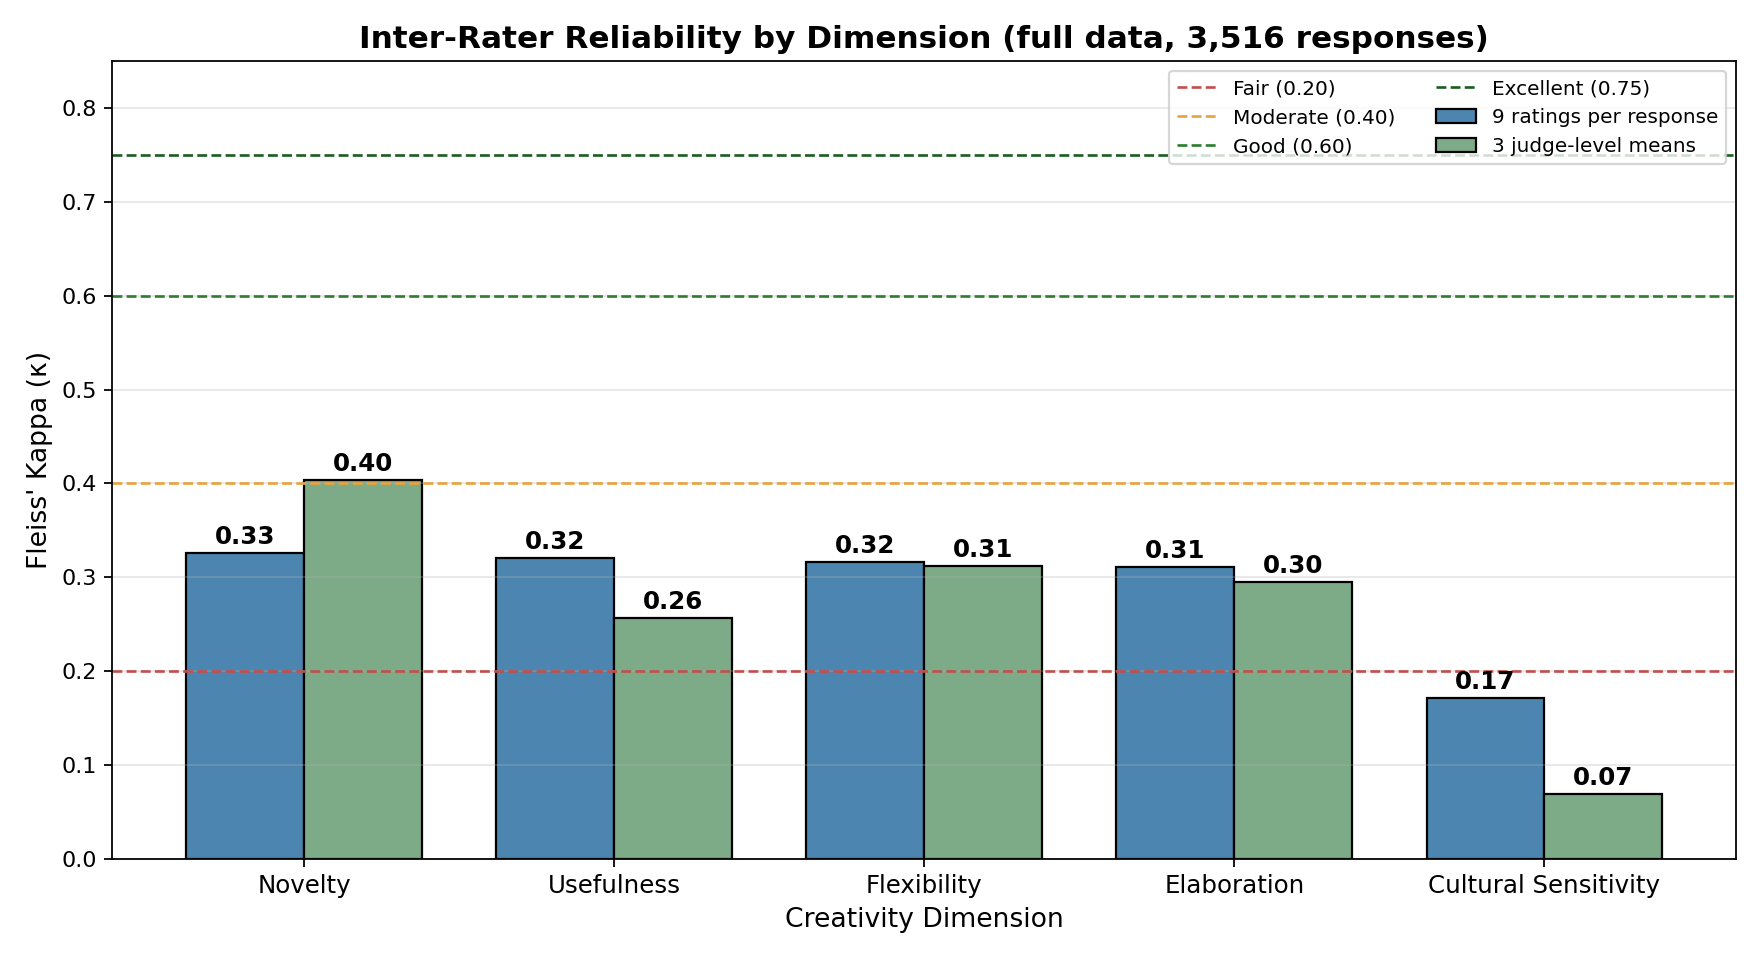
\includegraphics[width=0.85\textwidth]{figures_v2/figure7_inter_rater_reliability.png}
\caption{Inter-rater reliability (Fleiss' $\kappa$) by dimension over the full dataset (3,516 responses), at both rater grains: nine individual ratings per response (blue) and three judge-level mean ratings (green). Dashed lines mark conventional interpretation thresholds. All four core dimensions fall in the fair band (0.20--0.40); only Cultural Sensitivity falls below it.}
\label{fig:inter_rater}
\end{figure}

Agreement was fair-to-moderate for the four core creativity dimensions (\(\kappa = 0.31\)--\(0.33\), statistically indistinguishable from one another) and poor for Cultural Sensitivity. An earlier subset-based estimate (\(\kappa = 0.68\) for Novelty, 35 responses) proved unstable---across random 35-response subsets \(\kappa\) for Novelty ranges from 0.16 to 0.71 (median 0.39)---so we report full-data values throughout. Because reliability does not privilege any single core dimension, our focus on Novelty is theoretical: it is the construct at the center of our research question. Figure~\ref{fig:inter_rater} visualizes both rater grains against the conventional interpretation thresholds. Findings for the other dimensions are reported as exploratory given their limited reliability.

\subsection{Statistical Analysis}

\subsubsection{Effect Size Calculation}

Cohen's $d$ was calculated with 95\% bootstrap confidence intervals (5,000 resamples) using the formula:

\begin{equation}
d = \frac{\bar{x}_1 - \bar{x}_2}{s_{\text{pooled}}}, \quad s_{\text{pooled}} = \sqrt{\frac{(n_1-1)s_1^2 + (n_2-1)s_2^2}{n_1 + n_2 - 2}}
\end{equation}

Effect sizes were interpreted as negligible ($|d| < 0.2$), small ($0.2 \le |d| < 0.5$), medium ($0.5 \le |d| < 0.8$), or large ($|d| \ge 0.8$).

\subsubsection{Inferential Statistics}

\begin{itemize}
    \item \textbf{Unit of Analysis:} All inferential statistics treat the response (the mean of its nine judge ratings) as the unit of analysis ($N = 3{,}516$ responses; approximately 100 per model $\times$ condition cell). Judge and prompt variation are within-response replications, not independent observations.
    \item \textbf{Two-Way ANOVA:} Used to test Persona $\times$ Region interactions for Novelty.
    \item \textbf{Moderation Analysis:} Tested whether training region (Eastern vs. Western) moderates persona effects using OLS regression, with Bayes Factor calculated to quantify evidence strength (Rouder et al., 2009).
    \item \textbf{Domain Analysis:} Calculated effect sizes for each persona across the four problem domains.
    \item \textbf{False Discovery Rate (FDR):} Benjamini-Hochberg correction applied to the family of pure persona effect tests (Appendix A.8); significance elsewhere is assessed by bootstrap confidence-interval exclusion.
\end{itemize}

\subsubsection{Economic Analysis}

\begin{itemize}
    \item \textbf{Cost-Performance Frontier:} Plotted performance gain (Cohen's d for Novelty) against cost per 1M output tokens.
    \item \textbf{Efficiency Gain Ratio (EGR):} Defined as:
    \begin{equation}
    EGR = \frac{\text{Performance}_{\text{small+persona}} / \text{Performance}_{\text{large}}}{\text{Cost}_{\text{small}} / \text{Cost}_{\text{large}}}
    \end{equation}
    The performance value is the Novelty score.
    Thresholds: $EGR > 1.0 =$ economic value, $EGR > 2.0 =$ strong value, $EGR > 5.0 =$ exceptional value, $EGR > 10.0 =$ transformative value.
    The metric assumes comparable output token counts across models; Gemini's reasoning traces violate this assumption (Section 4.7), so Gemini is excluded from the economic analysis. Because EGR ratios a 1--5 scale mean against a price ratio, it can label significantly \emph{harmful} combinations as valuable (e.g., Qwen with Culture\_11, $d = -0.638$, would score EGR $= 3.99$); we therefore report EGR only for combinations with statistically significant positive gains.
\end{itemize}

\subsubsection{Robustness Checks}

\begin{itemize}
    \item \textbf{Power Analysis:} Post-hoc power calculated using TTestIndPower.
    \item \textbf{Leave-One-Out Sensitivity:} Removed each model sequentially to test result stability.
    \item \textbf{Outlier Detection:} Isolation Forest (contamination $= 0.1$) identified extreme responses.
    \item \textbf{Generalizability:} Train-test split (80/20 by problem) validated across-problem consistency.
    \item \textbf{ANOVA Assumptions:} Shapiro-Wilk test for normality of residuals; Levene's test for homogeneity of variance (results reported in Section 4.2.1).
\end{itemize}

\subsection{Validity and Reliability}

Internal validity was ensured through controlled variables: identical problem set, judge models, and evaluation protocol across all conditions. External validity was supported by diverse model selection (7 models, Eastern/Western, varying sizes) and multiple problem domains. Reliability was ensured through inter-rater reliability assessment (Fleiss' Kappa) and transparent, replicable protocol.

\subsection{Code and Data Availability}

 Statistics code and data are available at: https://github.com/youssef-hariri/persona-model-fit.

\section{Results}

Based on the inter-rater reliability analysis (Section 3.6), which showed fair-to-moderate agreement for the four core dimensions (\(\kappa = 0.31\)--\(0.33\)) and poor agreement for Cultural Sensitivity (\(\kappa = 0.17\)), we focus our primary analysis on Novelty, the dimension central to our research question. Findings for Usefulness, Flexibility, Elaboration, and Cultural Sensitivity are reported in the Appendix as exploratory.

\subsection{Overall Effectiveness and Model-Dependent Patterns}

\subsubsection{Overview of Model Performance}

We evaluated seven large language models across five conditions (three cultural personas and two baselines) on 100 problems spanning four domains: Creative, General Knowledge, Instruction, and Reasoning. Table~\ref{tab:means_novelty} presents the mean Novelty scores (1-5 scale) for the three persona conditions and the large baseline (Small Baseline means appear in Appendix A.8). Standard deviations and sample sizes are reported at the response level, the unit of all inferential analyses in this paper.

\begin{table}[H]
\centering
\caption{Mean Novelty Scores (1-5) by Model and Condition}
\label{tab:means_novelty}
\begin{tabular}{lcccc}
\toprule
\multirow{2}{*}{Model} & \multicolumn{4}{c}{Condition} \\
\cmidrule(lr){2-5}
 & Culture\_5 & Culture\_Expert & Culture\_11 & Large Baseline \\
\midrule
\textbf{Western Models} \\
Claude & 3.81 (0.64) & 3.14 (1.06) & 2.89 (0.95) & 2.84 (1.09) \\
Gemini & 1.49 (0.73) & 1.45 (0.56) & 1.21 (0.34) & 1.41 (0.55) \\
GPT & 3.22 (0.99) & 3.00 (1.04) & 2.88 (1.02) & 2.64 (1.06) \\
Llama & 2.50 (0.74) & 2.34 (0.68) & 1.97 (0.68) & 2.29 (0.86) \\
Mistral & 2.50 (0.74) & 2.29 (0.74) & 1.95 (0.80) & 2.36 (0.85) \\
\midrule
\textbf{Eastern Models} \\
DeepSeek & 3.35 (1.02) & 3.14 (1.03) & 2.64 (1.00) & 2.64 (1.13) \\
Qwen & 2.63 (0.71) & 2.51 (0.69) & 2.26 (0.72) & 2.83 (1.05) \\
\bottomrule
\end{tabular}
\caption*{\footnotesize Response-level means and standard deviations (each response is the mean of nine judge ratings). n = 100 responses per cell except GPT Culture\_5 = 120 (20 of the 100 problems were generated twice; averaging duplicates to one value per problem leaves the conclusion unchanged, $d = 0.624$ vs. $0.570$) and Gemini/Mistral Large Baseline = 99. \textbf{Note:} Gemini shows notably smaller standard deviations (e.g., 0.34 for Culture\_11 vs. 0.64--1.13 for others), indicating consistently low scores with little variation across responses.}
\end{table}

Figure~\ref{fig:barplot_novelty} visualizes these scores, revealing substantial variation across models and conditions.

\begin{figure}[H]
\centering
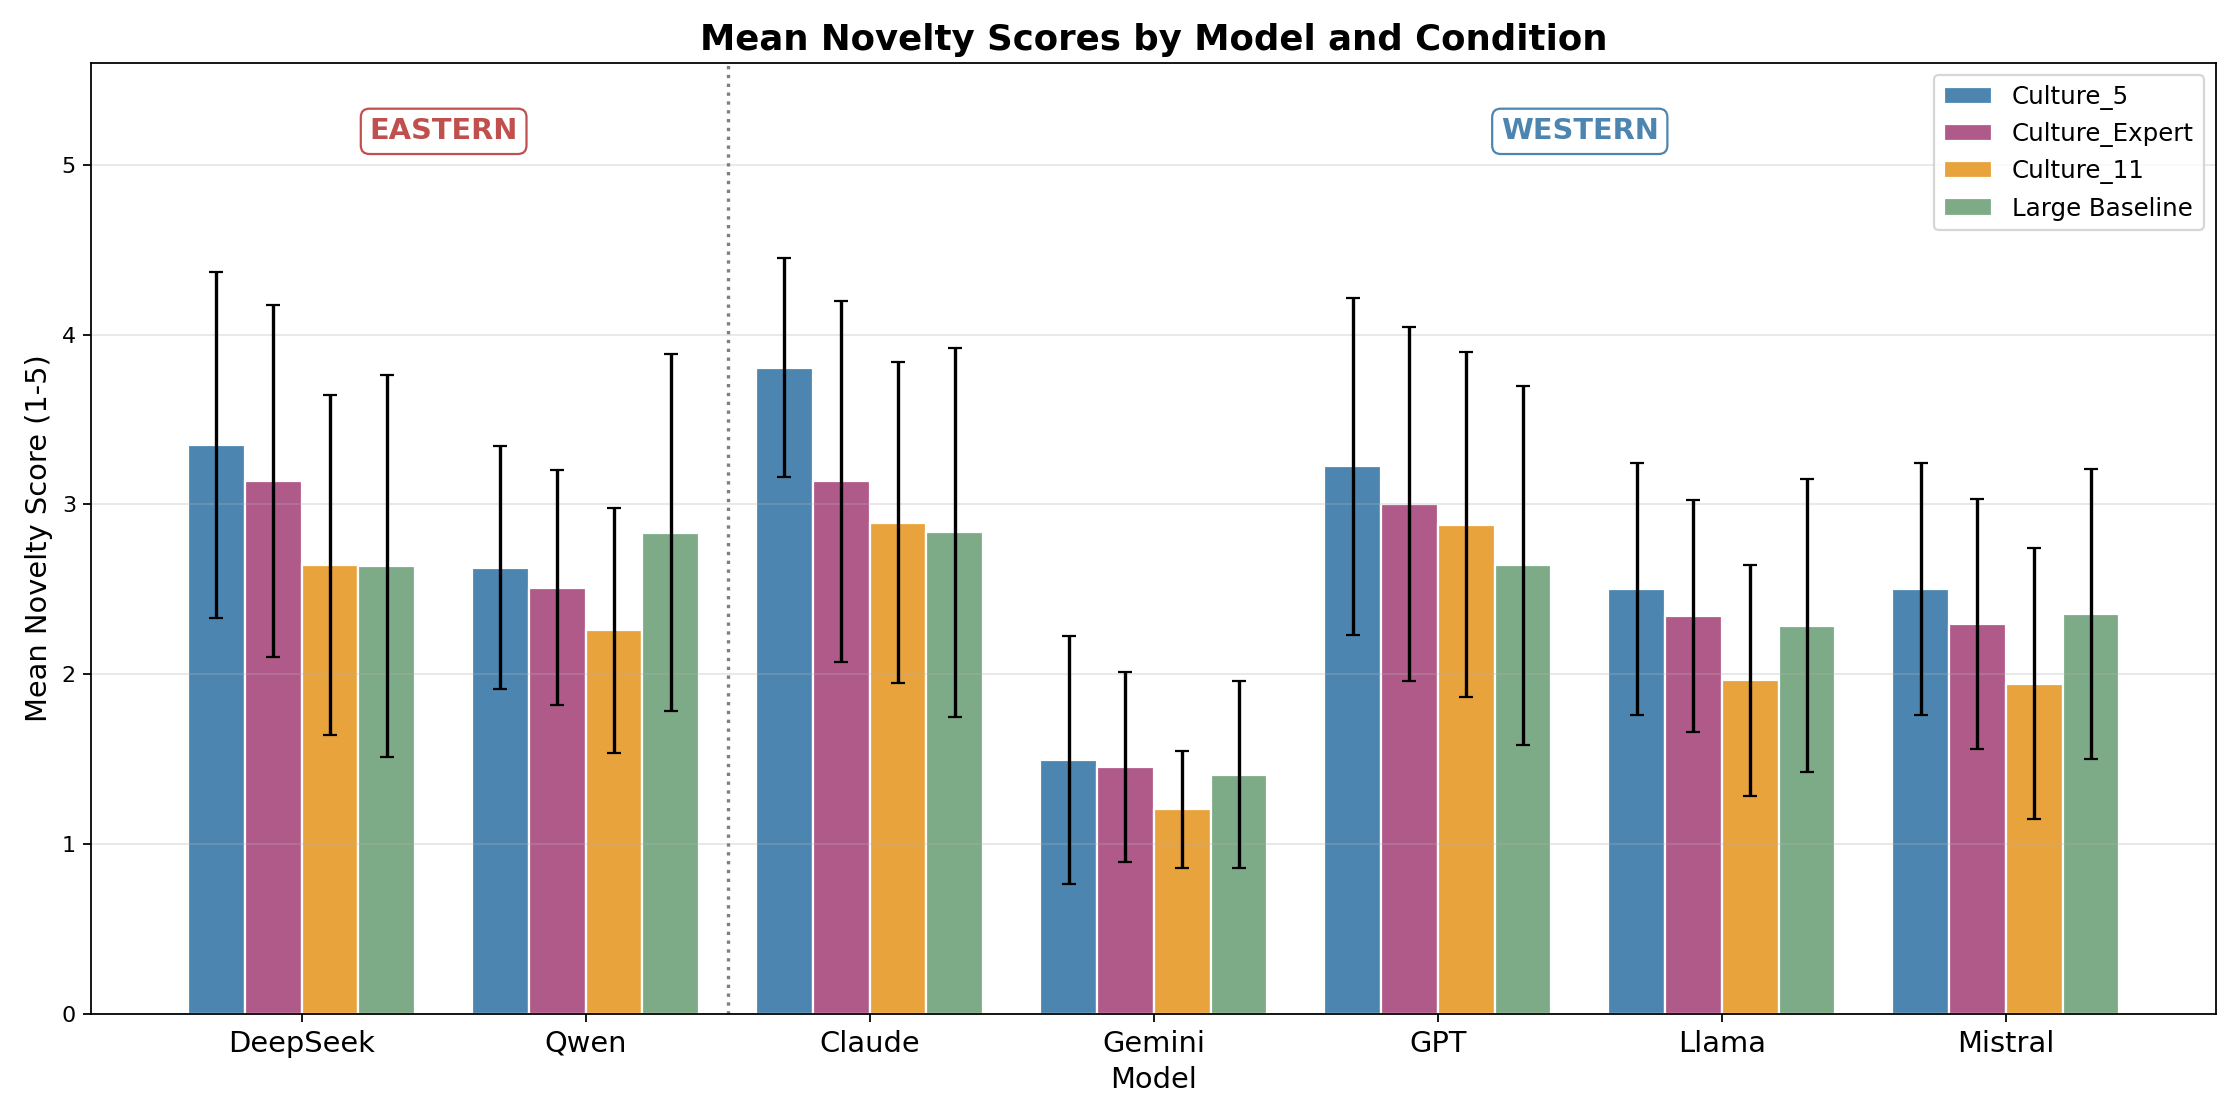
\includegraphics[width=0.8\columnwidth]{figures_v2/figure1_performance_barplot_novelty.png}
\caption{Mean Novelty scores by model and condition. Error bars represent $\pm1$ standard deviation (response level). Bars are colored by condition; models are grouped by training region (Eastern: DeepSeek, Qwen; Western: the remaining five), separated by the dotted line.}
\label{fig:barplot_novelty}
\end{figure}

Claude achieved the highest mean Novelty in three of four conditions ($M = 3.10$, $SD = 1.05$ across conditions); Qwen's unsteered large model matched it ($2.83$ vs. $2.84$). Gemini performed substantially lower ($M = 1.39$ across conditions), approximately 0.9 points below the next-lowest models (Llama, $M = 2.26$; Mistral, $M = 2.27$). Claude showed the largest improvement from personas, with Culture\_5 outperforming its large baseline by 0.97 points ($+34.2\%$); DeepSeek showed the second-largest improvement ($+0.71$ points, $+27.1\%$). In contrast, Qwen showed the largest degradation with Culture\_11, dropping 0.58 points ($-20.3\%$) below baseline.

\subsubsection{Effect Sizes with Bootstrap Confidence Intervals}

To quantify the practical significance of persona effects, we calculated Cohen's $d$ effect sizes comparing each persona to the large baseline at the response level (100 responses per cell), with 95\% bootstrap confidence intervals (5,000 resamples). Positive values indicate improvement over baseline; negative values indicate degradation. Effect sizes are interpreted as negligible ($|d| < 0.2$), small ($0.2 \le |d| < 0.5$), medium ($0.5 \le |d| < 0.8$), or large ($|d| \ge 0.8$).

Table~\ref{tab:effects_complete} presents the complete effect sizes with confidence intervals for all model-persona combinations.

\begin{table}[H]
\centering
\caption{Complete Cohen's d Effect Sizes for Novelty with 95\% Bootstrap CIs}
\label{tab:effects_complete}
\begin{tabular}{lcccc}
\toprule
Model & Persona & d & 95\% CI & Magnitude \\
\midrule
Claude & Culture\_5 & 1.087 & [0.800, 1.417] & Large \\
Claude & Culture\_Expert & 0.281 & [0.012, 0.574] & Small \\
Claude & Culture\_11 & 0.056 & [-0.213, 0.337] & Negligible \\
DeepSeek & Culture\_5 & 0.664 & [0.384, 0.993] & Medium \\
DeepSeek & Culture\_Expert & 0.464 & [0.186, 0.770] & Small \\
DeepSeek & Culture\_11 & 0.006 & [-0.264, 0.285] & Negligible \\
GPT & Culture\_5 & 0.570 & [0.308, 0.868] & Medium \\
GPT & Culture\_Expert & 0.344 & [0.070, 0.647] & Small \\
GPT & Culture\_11 & 0.231 & [-0.043, 0.521] & Small \\
Llama & Culture\_5 & 0.271 & [-0.006, 0.561] & Small \\
Llama & Culture\_Expert & 0.076 & [-0.196, 0.363] & Negligible \\
Llama & Culture\_11 & -0.412 & [-0.693, -0.131] & Small \\
Mistral & Culture\_5 & 0.186 & [-0.094, 0.461] & Negligible \\
Mistral & Culture\_Expert & -0.077 & [-0.367, 0.203] & Negligible \\
Mistral & Culture\_11 & -0.496 & [-0.816, -0.215] & Small \\
Qwen & Culture\_5 & -0.229 & [-0.504, 0.040] & Small \\
Qwen & Culture\_Expert & -0.365 & [-0.642, -0.097] & Small \\
Qwen & Culture\_11 & -0.638 & [-0.925, -0.366] & Medium \\
Gemini & Culture\_5 & 0.131 & [-0.154, 0.396] & Negligible \\
Gemini & Culture\_Expert & 0.076 & [-0.205, 0.355] & Negligible \\
Gemini & Culture\_11 & -0.443 & [-0.701, -0.182] & Small \\
\bottomrule
\end{tabular}
\caption*{\footnotesize Response-level effect sizes (each response is the mean of nine judge ratings). Magnitude: negligible ($|d| < 0.2$), small ($0.2 \le |d| < 0.5$), medium ($0.5 \le |d| < 0.8$), large ($|d| \ge 0.8$). Bootstrap confidence intervals (5,000 resamples) that do not contain zero indicate statistical significance (11/21 comparisons).}
\end{table}

\begin{figure}[H]
\centering
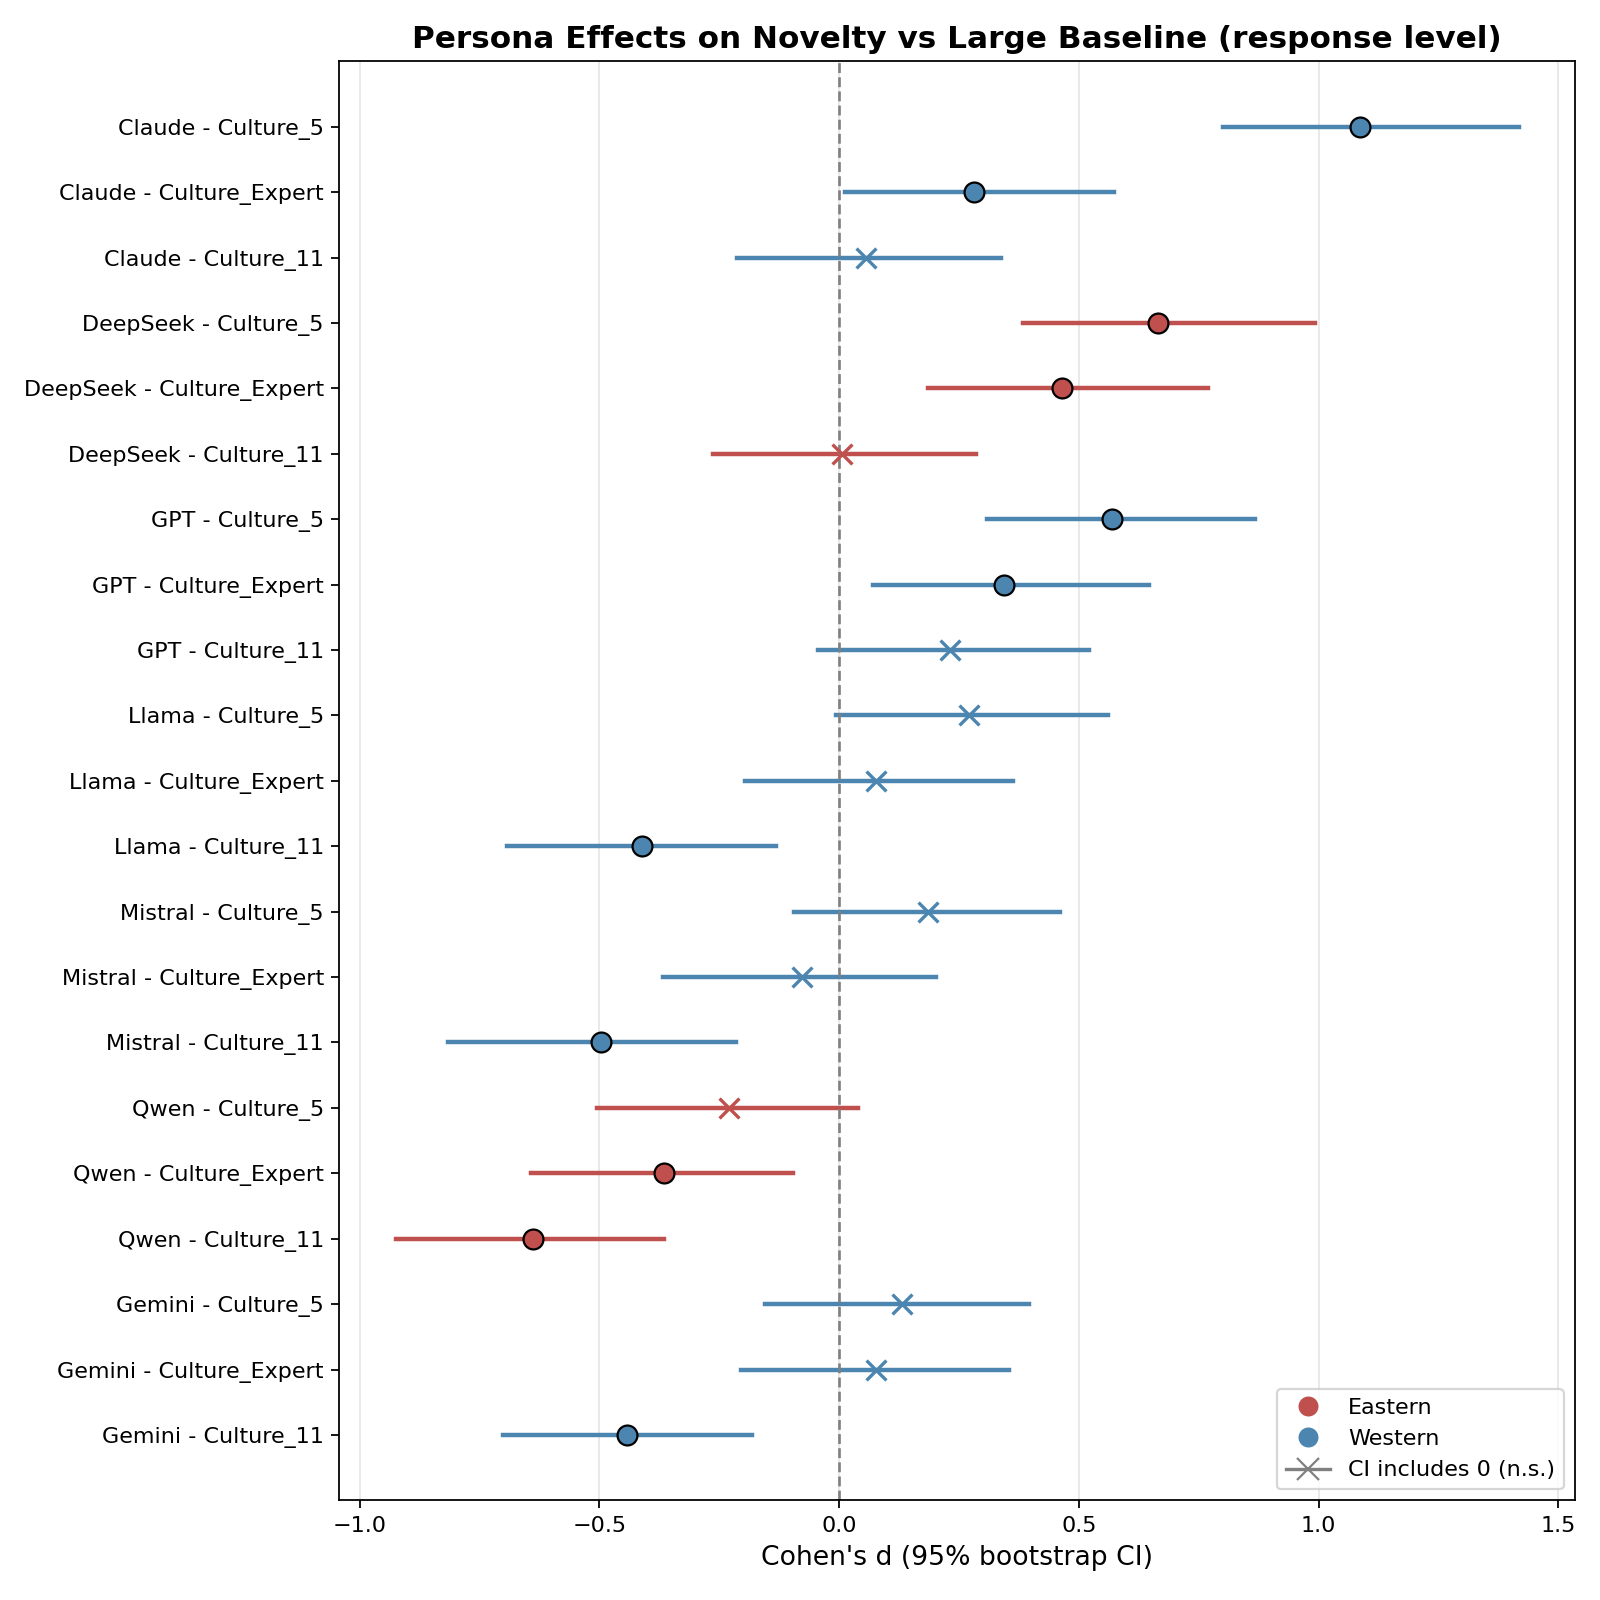
\includegraphics[width=0.9\textwidth]{figures_v2/figure2_forest_plot_novelty.png}
\caption{Forest plot of response-level Cohen's d effect sizes for Novelty with 95\% bootstrap confidence intervals. Red points indicate Eastern models (DeepSeek, Qwen); blue points indicate Western models; crosses mark intervals that include zero (non-significant). The vertical dashed line represents no effect.}
\label{fig:forest_novelty}
\end{figure}

Three distinct patterns emerge:

\textbf{Consistently Positive:} Claude and DeepSeek show positive effects across most personas. Claude with Culture\_5 achieves a large positive effect ($d = 1.087$), the largest in the study. DeepSeek with Culture\_5 shows a medium positive effect ($d = 0.664$). GPT shows significant small-to-medium positive effects for Culture\_5 ($d = 0.570$) and Culture\_Expert ($d = 0.344$); its Culture\_11 effect is not significant ($d = 0.231$, CI includes zero).

\textbf{Consistently Negative:} Qwen shows negative effects across all personas, significant for Culture\_Expert ($d = -0.365$) and for Culture\_11 ($d = -0.638$, medium). Mistral shows mixed but predominantly negative effects, with Culture\_11 showing a significant small negative effect ($d = -0.496$).

\textbf{Neutral or Mixed:} Llama shows a non-significant small positive effect for Culture\_5 ($d = 0.271$) but a significant small negative effect for Culture\_11 ($d = -0.412$). Gemini shows negligible, non-significant effects for Culture\_5 and Culture\_Expert ($|d| < 0.14$); its Culture\_11 effect is negative and significant ($d = -0.443$), although Gemini's results carry the measurement caveat of Section 4.7.

\subsubsection{Key Takeaway}

Persona effectiveness on Novelty is not universal. Claude and DeepSeek benefit substantially; Qwen and Mistral are harmed; Gemini is largely unresponsive, with a significant negative Culture\_11 effect that should be read in light of its evaluation anomaly (Section 4.7). This heterogeneity motivates our investigation of the factors that moderate persona effectiveness.
\subsection{Regional Moderation and Cross-Architectural Variation}

\subsubsection{Two-Way ANOVA (Persona $\times$ Region)}

A two-way ANOVA with persona (4 levels) and training region (2 levels: Eastern vs. Western) as fixed factors, computed at the response level, revealed strong main effects of persona and region but no interaction ($F(3, 2810) = 0.89$, $p = 0.445$), indicating that persona effects do not vary systematically by training region. Table~\ref{tab:anova_novelty} presents the full ANOVA results. Assumption checks indicated non-normal residuals (Shapiro-Wilk $p < 0.001$) and heterogeneity of variance (Levene $p = 0.003$); with 2,818 observations the F-tests are robust to these violations, and the key inferences in this paper rely on bootstrap confidence intervals rather than ANOVA p-values.

\begin{table}[H]
\centering
\caption{Two-Way ANOVA Results for Novelty (Persona $\times$ Region)}
\label{tab:anova_novelty}
\begin{tabular}{lcccc}
\toprule
Source & SS & df & F & p \\
\midrule
Persona & 112.31 & 3 & 35.75 & $<$0.001 \\
Region & 64.41 & 1 & 61.51 & $<$0.001 \\
Persona $\times$ Region & 2.80 & 3 & 0.89 & 0.445 \\
Residual & 2942.46 & 2810 & & \\
\bottomrule
\end{tabular}
\caption*{\footnotesize Response-level analysis ($n = 2{,}818$ responses). No persona $\times$ region interaction. An earlier version of this table, computed on a superseded data extract, reported a marginal interaction ($p = 0.052$) that matched neither the rating-level ($p = 0.0004$) nor the response-level ($p = 0.445$) analysis of the released data; it has been corrected.}
\end{table}

\subsubsection{Moderation Analysis with Bayes Factor}

To test whether training region moderates persona effects, we conducted a moderation analysis with region (Eastern vs. Western) as the moderator. At the response level, region did not moderate persona effects ($t = -1.27$, $p = 0.21$ for the persona $\times$ region interaction), consistent with the Bayes Factor ($BF = 0.331$), which provides anecdotal evidence against the moderation hypothesis. Table~\ref{tab:moderation_novelty} presents the full moderation results.

\begin{table}[H]
\centering
\caption{Moderation Analysis for Novelty (Training Region $\times$ Persona)}
\label{tab:moderation_novelty}
\begin{tabular}{lcccc}
\toprule
Source & Coefficient & SE & t & p \\
\midrule
Constant & 2.307 & 0.047 & 49.46 & $<$0.001 \\
Is Eastern & 0.428 & 0.087 & 4.91 & $<$0.001 \\
Is Persona & 0.147 & 0.054 & 2.73 & 0.006 \\
Eastern $\times$ Persona & -0.127 & 0.101 & -1.27 & 0.206 \\
\bottomrule
\end{tabular}
\caption*{\footnotesize Response-level OLS ($n = 2{,}818$ responses). Bayes Factor for interaction: $BF = 0.331$ (anecdotal evidence against moderation). Eastern models: DeepSeek, Qwen; Western models: Claude, Gemini, GPT, Llama, Mistral.}
\end{table}

Descriptively, Western models show slightly larger mean effects for the positive personas (Culture\_5: $d = +0.449$ Western vs. $+0.218$ Eastern; Culture\_Expert: $+0.140$ vs. $+0.050$), while Culture\_11 is negative in both regions ($-0.213$ Western, $-0.316$ Eastern); none of these differences is significant (Culture\_Expert $\times$ East: $t = 0.87$, $p = 0.38$; HC3-robust $p = 0.35$). The apparent significance of regional moderation at the rating level ($t = -3.41$ for the binary specification) is an artifact of treating the nine judge ratings of each response as independent observations, and an earlier report that Eastern models respond more strongly to Culture\_Expert does not survive correction at either grain.

\newpage
\subsubsection{Model Clustering}

Figure~\ref{fig:mds_novelty} shows multidimensional scaling (MDS) of model performance profiles across all conditions.

\begin{figure}[H]
\centering
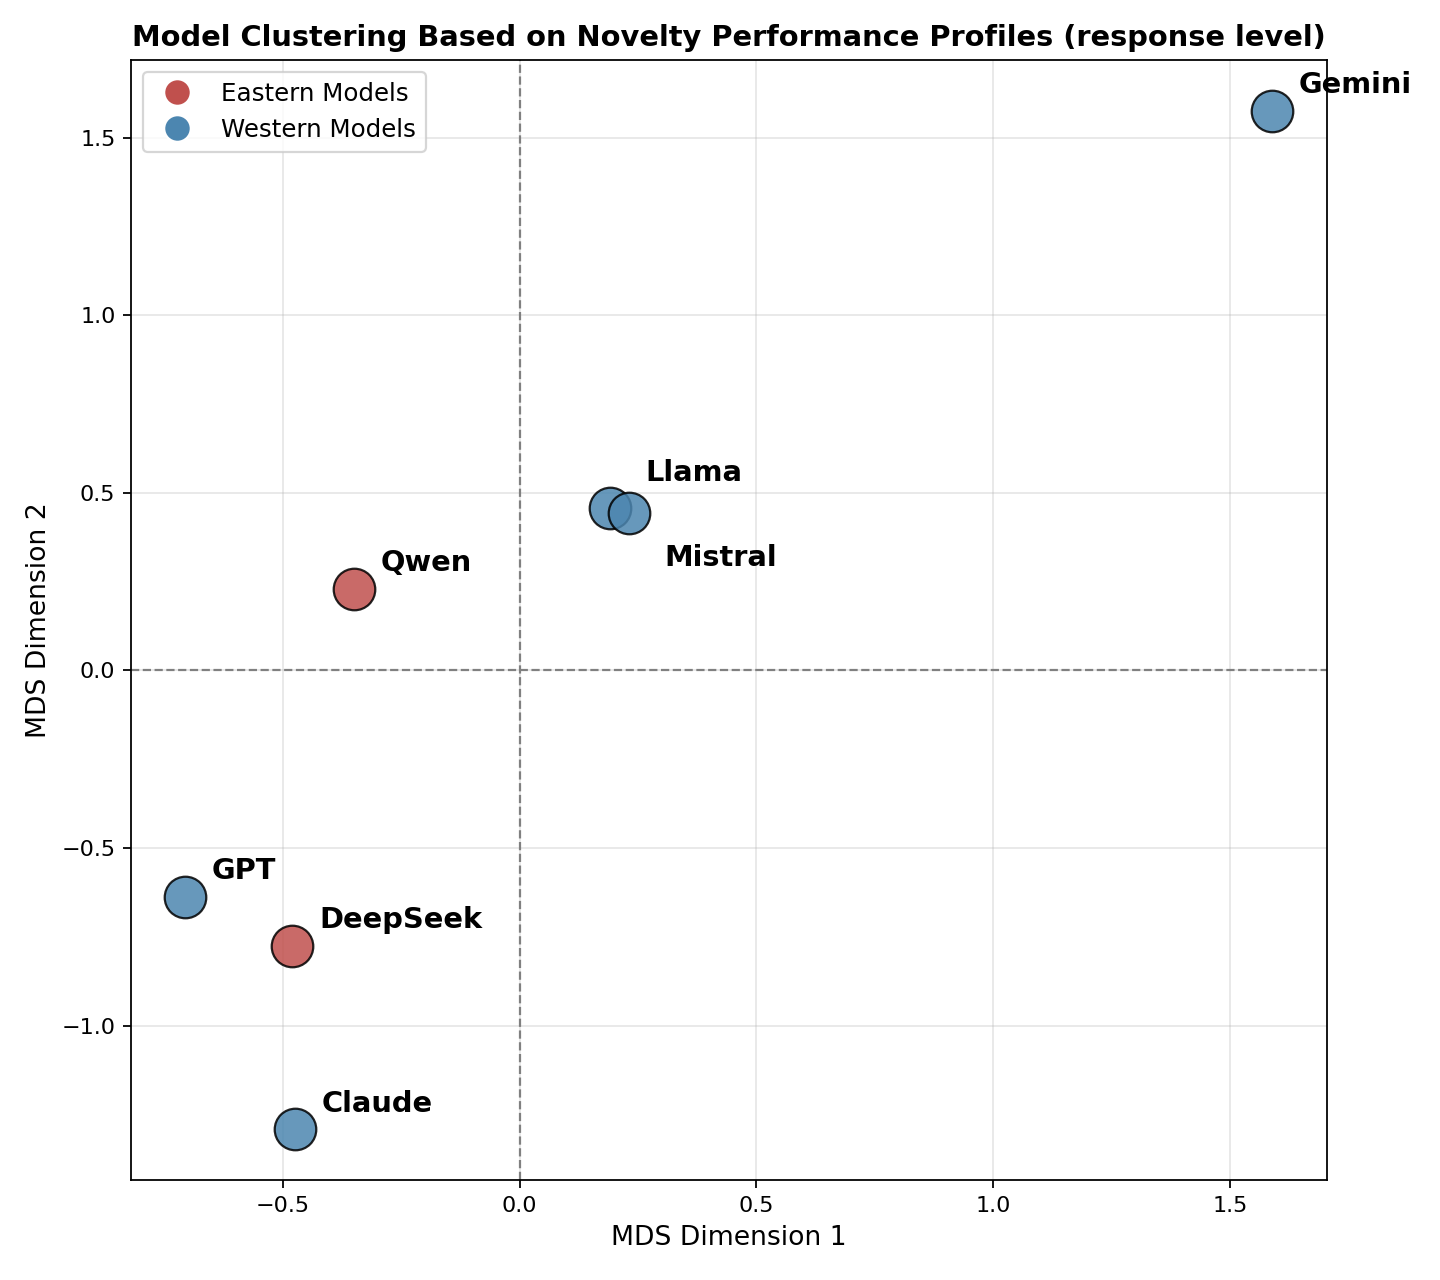
\includegraphics[width=0.9\textwidth]{figures_v2/figure4_mds_plot_novelty.png}
\caption{Multidimensional scaling (MDS) of model Novelty performance profiles. Eastern models (DeepSeek, Qwen) shown in red; Western models in blue.}
\label{fig:mds_novelty}
\end{figure}

The MDS analysis reveals clustering by performance profile rather than by training region: Claude, GPT, and DeepSeek form a high-Novelty group, while Llama, Mistral, and Qwen occupy a mid-range region. Gemini is a notable outlier, positioned far from all other models, reflecting its uniquely low Novelty scores across all conditions.

\subsubsection{Key Takeaway}

Persona effectiveness on Novelty depends on model architecture but shows no evidence of regional moderation at the response level (interaction $p = 0.445$; Bayes Factor = 0.331). Earlier indications that Eastern models respond more strongly to cultural personas were artifacts of rating-level analysis.

\subsection{Domain-Specific Effects}

The effectiveness of cultural personas on Novelty varies by problem domain. The 100 sets of problems used in this research follow the original dataset categorization of the problems into four domains: Creative, General Knowledge, Instruction, and Reasoning.

\begin{figure}[H]
\centering
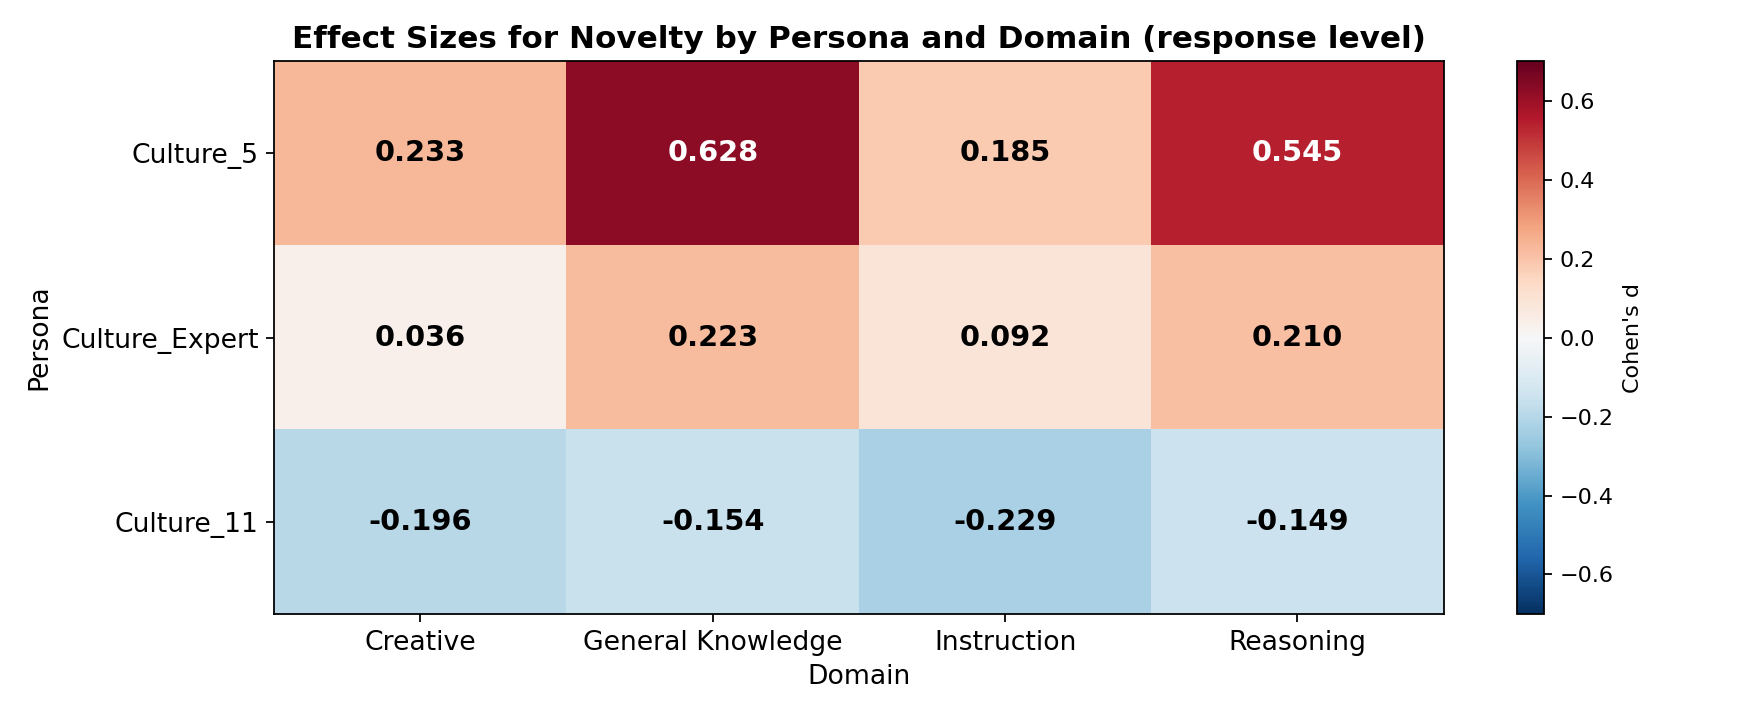
\includegraphics[width=0.9\textwidth]{figures_v2/figure3_domain_heatmap_novelty.png}
\caption{Response-level effect sizes (Cohen's d) for Novelty by persona and problem domain, models pooled. Blue indicates negative effects (harmful), red indicates positive effects (beneficial).}
\label{fig:domain_heatmap_novelty}
\end{figure}

Table~\ref{tab:domain_novelty} presents the effect sizes numerically.

\begin{table}[H]
\centering
\caption{Domain-Specific Effect Sizes for Novelty}
\label{tab:domain_novelty}
\begin{tabular}{lcccc}
\toprule
\textbf{Persona} & \textbf{Creative} & \textbf{General Knowledge} & \textbf{Instruction} & \textbf{Reasoning} \\
\midrule
Culture\_5 & 0.233 & \textbf{0.628} & 0.185 & 0.545 \\
Culture\_Expert & 0.036 & \textbf{0.223} & 0.092 & 0.210 \\
Culture\_11 & -0.196 & -0.154 & -0.229 & -0.149 \\
\bottomrule
\end{tabular}
\caption*{\footnotesize Response-level effect sizes, models pooled. Bold indicates largest effect for each persona. All Culture\_11 effects are negative. The pattern is unchanged when Gemini is excluded (Culture\_5: $d = 0.287/0.732/0.240/0.647$ for Creative/General Knowledge/Instruction/Reasoning).}
\end{table}

\textbf{Culture\_5} performs best on General Knowledge problems ($d = 0.628$) and Reasoning problems ($d = 0.545$), with smaller effects on Creative ($d = 0.233$) and Instruction ($d = 0.185$).

\textbf{Culture\_Expert} shows small positive effects across all domains, with the largest effect on General Knowledge ($d = 0.223$), followed closely by Reasoning ($d = 0.210$).

\textbf{Culture\_11} harms Novelty across all domains, with the most negative effect on Instruction ($d = -0.229$) and Creative ($d = -0.196$).

\subsubsection{Key Takeaway}

Domain matters for persona effectiveness on Novelty. Culture\_5 is most effective on General Knowledge and Reasoning problems. Culture\_11 consistently harms Novelty regardless of domain (See Figure~\ref{fig:domain_heatmap_novelty}).

\subsection{Economic Implications: Cost-Performance Trade-offs and Efficiency Gains}

\subsubsection{Positive Cases: Performance Gains with Cost Savings}

Six model-persona combinations achieve statistically significant Novelty gains (95\% bootstrap CI excludes zero) with small-model cost at or below their own large model's cost. Table~\ref{tab:economics_novelty} presents the cost-performance landscape for these combinations.

\begin{table}[H]
\centering
\caption{Cost-Performance Analysis for Novelty: Small Models with Personas}
\label{tab:economics_novelty}
\begin{tabular}{lcccccc}
\toprule
Model & Persona & Effect Size ($d$) & \multicolumn{2}{c}{Cost (\$/1M tokens)} & Cost \\
& & & Small & Large & Savings \\
\midrule
GPT & Culture\_5 & 0.570 & \$2.00 & \$15.00 & 87\% \\
GPT & Culture\_Expert & 0.344 & \$2.00 & \$15.00 & 87\% \\
Claude & Culture\_5 & 1.087 & \$15.00 & \$25.00 & 40\% \\
Claude & Culture\_Expert & 0.281 & \$15.00 & \$25.00 & 40\% \\
DeepSeek & Culture\_5 & 0.664 & \$0.42 & \$0.42 & 0\% \\
DeepSeek & Culture\_Expert & 0.464 & \$0.42 & \$0.42 & 0\% \\
\bottomrule
\end{tabular}
\caption*{\footnotesize Output token costs per 1M tokens. Inclusion rule: statistically significant positive Novelty gain (Table~\ref{tab:effects_complete}) and small-model cost $\le$ large-model cost. DeepSeek shows cost parity (identical small/large costs) but significant positive performance gains.}
\end{table}

Figure~\ref{fig:cost_performance_frontier_novelty} visualizes these combinations.

\begin{figure}[H]
\centering
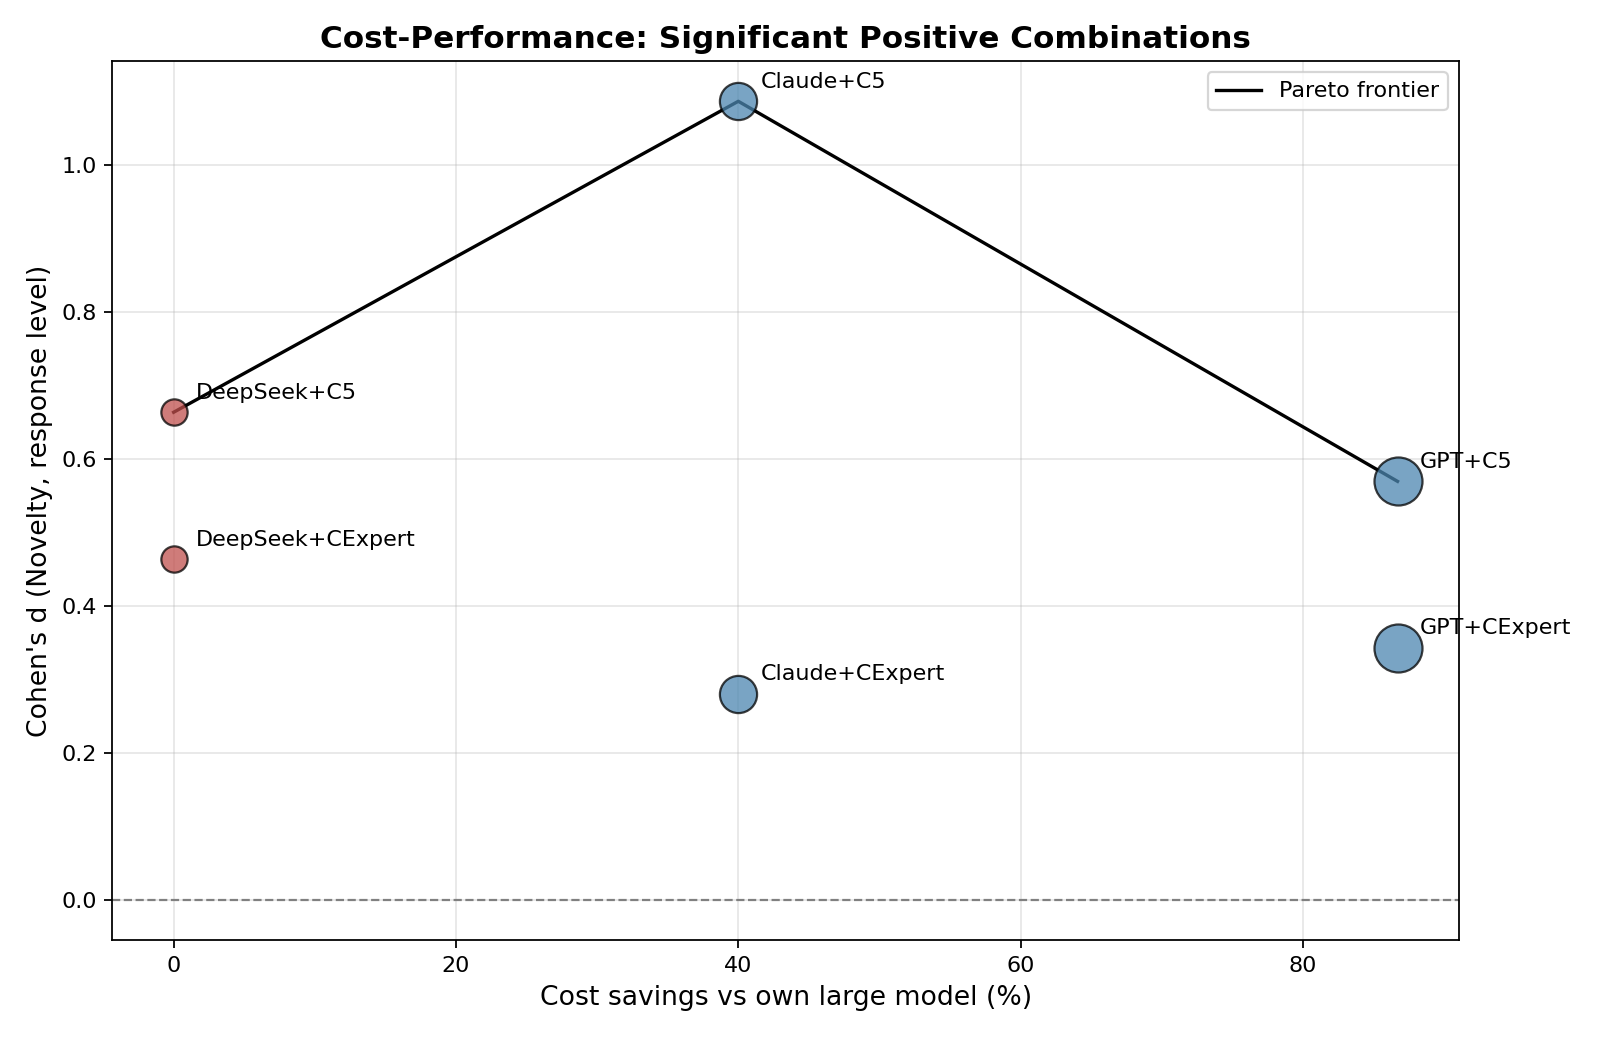
\includegraphics[width=0.85\textwidth]{figures_v2/figure6_cost_performance_frontier_novelty.png}
\caption{Cost-Performance Frontier for Novelty. Each point represents a small model with persona combination. Bubble size indicates cost savings. The Pareto frontier (black line) shows the optimal trade-off between cost savings and performance gain.}
\label{fig:cost_performance_frontier_novelty}
\end{figure}

Three distinct patterns emerge:

\textbf{GPT combinations} achieve the best balance, delivering significant positive performance gains ($d = 0.344$ to $0.570$) with exceptional cost savings (87\%), placing them firmly in the optimal region.

\textbf{Claude with Culture\_5} achieves the largest performance gain ($d = 1.087$) with substantial cost savings (40\%), approaching the optimal region.

\textbf{DeepSeek combinations} achieve significant positive performance gains ($d = 0.464$ to $0.664$) but offer no cost savings (0\%), placing them in the high-performance, cost-parity quadrant.

\subsubsection{Cross-Model Value}

Beyond within-family comparisons, small models with personas can outperform larger models from competing providers. DeepSeek with Culture\_5 ($d = 0.664$) achieves comparable Novelty performance to Claude Opus at 60× lower cost (\$0.42 vs. \$25.00 per 1M output tokens). GPT with Culture\_5 ($d = 0.570$) achieves similar performance at 12.5× lower cost (\$2.00 vs. \$25.00).

\subsubsection{Efficiency Gain Ratio (EGR)}

To unify performance and cost into a single metric, we calculated the Efficiency Gain Ratio (EGR):

\begin{equation}
EGR = \frac{\text{Novelty Score}_{\text{small+persona}} / \text{Novelty Score}_{\text{large}}}{\text{Cost}_{\text{small}} / \text{Cost}_{\text{large}}}
\end{equation}

An $EGR > 1.0$ indicates economic value; $EGR > 2.0$ indicates strong value; $EGR > 5.0$ indicates exceptional value; $EGR > 10.0$ indicates transformative value.

Table~\ref{tab:egr_complete} presents the complete EGR results for all model-persona combinations with statistically significant positive performance gains.

\begin{table}[H]
\centering
\caption{Complete EGR Results for Novelty (Positive Combinations)}
\label{tab:egr_complete}
\begin{tabular}{lcccc}
\toprule
Model & Persona & Effect Size ($d$) & Cost Savings & EGR \\
\midrule
GPT & Culture\_5 & 0.570 & 87\% & 9.15 \\
GPT & Culture\_Expert & 0.344 & 87\% & 8.53 \\
Claude & Culture\_5 & 1.087 & 40\% & 2.24 \\
Claude & Culture\_Expert & 0.281 & 40\% & 1.84 \\
DeepSeek & Culture\_5 & 0.664 & 0\% & 1.27 \\
DeepSeek & Culture\_Expert & 0.464 & 0\% & 1.19 \\
\bottomrule
\end{tabular}
\caption*{\footnotesize EGR $> 1$ indicates economic value; $> 2$ strong value; $> 5$ exceptional value. DeepSeek shows cost parity (0\% savings) but positive performance gains.}
\end{table}

\begin{figure}[H]
\centering
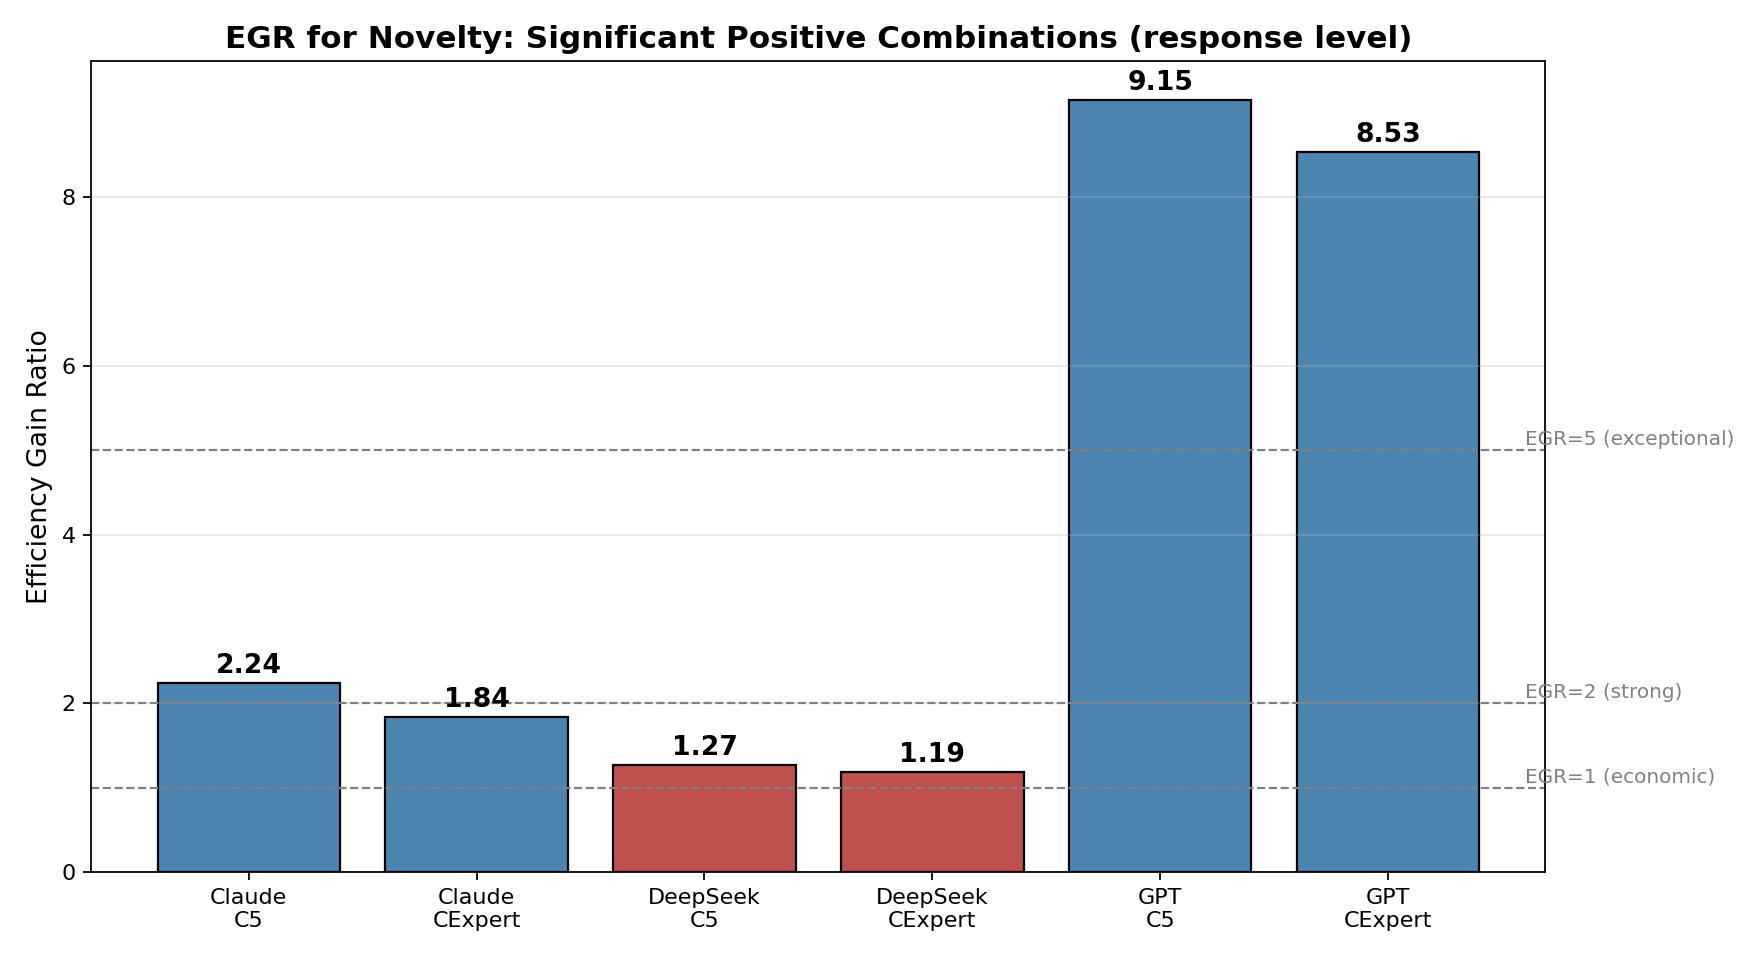
\includegraphics[width=0.85\textwidth]{figures_v2/figure5_egr_bar_chart_novelty.png}
\caption{Efficiency Gain Ratio (EGR) for Novelty by model and persona. Threshold lines indicate value tiers: $EGR > 1$ (economic value), $EGR > 2$ (strong value), $EGR > 5$ (exceptional value).}
\label{fig:egr_bar_novelty}
\end{figure}

\textbf{GPT combinations} achieve exceptional economic value for Culture\_5 and Culture\_Expert (EGR = 8.53-9.15), delivering 87\% cost savings with significant positive performance gains.

\textbf{Claude with Culture\_5} achieves strong economic value (EGR = 2.24), delivering 40\% cost savings with a large performance gain ($d = 1.087$).

\textbf{DeepSeek combinations} achieve modest economic value (EGR = 1.19-1.27), with cost parity (0\% savings) but significant positive performance gains.

\subsubsection{Key Takeaway}

For the six significant combinations, small models with personas achieve superior Novelty performance at equal or lower cost (40-87\% savings for GPT and Claude; cost parity for DeepSeek). The EGR provides a unified metric for comparing economic efficiency across model families, with GPT achieving exceptional value and Claude achieving strong value (See Figure~\ref{fig:egr_bar_novelty}).

\subsection{Robustness Checks and Generalizability}

\subsubsection{Power Analysis}

Post-hoc power analysis at the response level showed mean power of 0.544, with 38.1\% of comparisons achieving sufficient power ($\ge 0.80$). Most comparisons are therefore underpowered at the correct unit of analysis: non-significant results should be read as insufficient evidence rather than as evidence of no effect, and the corrected confidence intervals (Table~\ref{tab:effects_complete}) widen accordingly.

\subsubsection{Leave-One-Out Sensitivity Analysis}

Leave-one-out sensitivity analysis confirmed that results are highly stable, with 19 of 21 effects (90\%) showing changes below the stability threshold of $|\Delta| < 0.1$ when removing any single model. The mean absolute change across all comparisons was $0.047$, with a maximum change of $0.117$ (observed when removing Claude for Culture\_5). Qwen had the largest average impact ($|\Delta| = 0.083$), followed by Claude ($|\Delta| = 0.065$), while Llama had the smallest impact ($|\Delta| = 0.018$). These findings indicate that while some models exert greater influence on the average effect sizes than others, no single model drives the observed patterns.

\subsubsection{Outlier Analysis}

Isolation Forest analysis (contamination = 0.1) flagged 10.0\% of responses as outliers (the contamination parameter fixes the flagged share). Removing them changed pooled persona effect sizes by at most $\Delta = 0.03$.

\subsubsection{Generalizability}

Train-test split (random 80/20 split by problem, seed 42) confirmed that the direction of persona effects generalizes to new problems:
- Culture\_5: train $d = 0.310$, test $d = 0.515$ ($\Delta = +0.205$)
- Culture\_Expert: train $d = 0.085$, test $d = 0.271$ ($\Delta = +0.186$)
- Culture\_11: train $d = -0.186$, test $d = -0.097$ ($\Delta = +0.089$)

Signs are consistent across splits for all three personas; magnitudes vary more at the response level (maximum $|\Delta| = 0.21$) because the test split contains only about 20 responses per condition.

\subsubsection{Key Takeaway}

Our findings are reliable, not driven by outliers, and generalize in direction to new problems. The leave-one-out sensitivity analysis confirms that while some models (particularly Qwen and Claude) exert greater influence on average effect sizes than others, no single model drives the observed patterns (19/21 changes $|\Delta| < 0.1$, maximum 0.117).

\subsection{Summary of Key Findings}

\begin{table}[H]
\centering
\caption{Summary of Key Findings for Novelty}
\label{tab:key_findings_novelty}
\begin{tabular}{p{3cm}p{9.5cm}}
\toprule
\textbf{Finding} & \textbf{Description} \\
\midrule
\textbf{1. Model-Dependent} & Persona effects on Novelty vary dramatically across models. Claude with Culture\_5 shows a large positive effect ($d = 1.087$); Qwen with Culture\_11 shows a medium negative effect ($d = -0.638$). \\
\midrule
\textbf{2. No Regional Moderation} & Training region did not moderate persona effects at the response level (interaction $p = 0.445$; Bayes Factor $= 0.331$). \\
\midrule
\textbf{3. Domain Specificity} & Culture\_5 performs best on General Knowledge ($d = 0.628$) and Reasoning ($d = 0.545$); Culture\_11 harms Novelty across all domains. \\
\midrule
\textbf{4. Economic Advantage} & Six small-model + persona combinations achieve significant gains at equal or lower cost (40-87\% savings for GPT and Claude; parity for DeepSeek). GPT achieves exceptional economic value (EGR up to 9.15); Claude achieves strong value (EGR $= 2.24$). \\
\midrule
\textbf{5. Robustness} & Results are stable (mean absolute change $= 0.047$, 19/21 changes $|\Delta| < 0.1$), generalize in direction to new problems, and are not driven by outliers. \\
\bottomrule
\end{tabular}
\end{table}

These five key findings are discussed in Section 5 alongside theoretical implications and practical guidance for practitioners.

\subsection{Anomaly: Gemini's Unique Response Format}

Gemini exhibited a response pattern not observed in any other model evaluated. Analysis of the raw outputs revealed that Gemini consistently wrapped its responses in special tags:

\begin{itemize}
    \item \texttt{<|begin\_of\_thought|>} and \texttt{<|end\_of\_thought|>} containing extensive internal reasoning chains
    \item \texttt{<|begin\_of\_solution|>} and \texttt{<|end\_of\_solution|>} containing the final answer
\end{itemize}

In contrast, all other models (Claude, GPT, DeepSeek, Llama, Mistral, Qwen) returned only the final answer without any reasoning traces or special tags.

This format inconsistency had two potential consequences for Gemini's evaluation:

\begin{enumerate}
    \item \textbf{Judge confusion}: The presence of extensive reasoning traces may have confused judge models, which were expecting only the final answer based on the response format of other models.
    \item \textbf{Task mismatch}: For structured extraction tasks (Problems 3-5), Gemini's output format deviated from the requested JSON schema, likely resulting in lower scores regardless of content quality.
\end{enumerate}

These factors explain Gemini's anomalously low Novelty scores ($M = 1.39$ vs. $2.67$ across all conditions for the other models; $M = 1.41$ vs. $2.60$ on the unsteered large baseline) and its largely negligible persona effects (Culture\_5 and Culture\_Expert $|d| < 0.14$, non-significant; Culture\_11 $d = -0.443$). Direct comparisons between Gemini and other models should be interpreted with caution, as the format inconsistency represents a measurement artifact rather than a genuine difference in model capability. Accordingly, Gemini is excluded from the economic analysis (Section 3.7.3) and from the domain-level robustness check (Section 4.3); pooled results include Gemini unless stated otherwise.


\section{Discussion}

This study evaluated whether small LLMs steered with cultural personas could outperform large LLMs on Novelty. Through a systematic evaluation of seven models across 100 problems, we find that persona effectiveness follows a contingency model rather than a universal rule. Inter-rater reliability was fair-to-moderate and statistically indistinguishable across the four core creativity dimensions (\(\kappa = 0.31\)--\(0.33\)); we focus on Novelty as the construct central to our research question.

\subsection{Theoretical Implications}

\subsubsection{Persona Capability as a Distinct Dimension of Intelligence}

Persona effects on Novelty vary dramatically across architectures. Claude with Culture\_5 showed a large positive effect (\(d = 1.087\)), while Qwen with Culture\_11 showed a medium negative effect (\(d = -0.638\)). This aligns with PersonaGym benchmark findings that persona capability is a distinct dimension of intelligence that does not scale linearly with model size (\cite{vinay_samuel_301ec4c0}). The dissociation whereby the far cheaper DeepSeek pair shows substantially larger persona effects than the Mistral pair confirms that neither cost nor raw parameter count is a reliable predictor of persona faithfulness.

Architectural differences may explain this heterogeneity. Mixture-of-Experts architectures excel in cultural knowledge retrieval, activating specialized "expert" neurons for different cognitive styles, while Dense Transformers maintain more consistent personas but exhibit stronger Western-default bias (\cite{reem_i__masoud_f9cde5f1, xinyu_zhang_c810e609}). The finding that DeepSeek, an MoE model far cheaper than its Western peers, achieves a medium positive effect with Culture\_5 (\(d = 0.664\)) suggests that MoE architectures may be particularly well-suited for persona-based steering on Novelty.

\subsubsection{Regional Moderation: Weak Evidence}

We found no evidence for regional moderation at the response level: the persona \(\times\) region interaction was non-significant in both the ANOVA (\(F(3, 2810) = 0.89\), \(p = 0.445\)) and the moderation regression (\(t = -1.27\), \(p = 0.21\)), in agreement with the Bayes Factor (\(BF = 0.331\)), which provides anecdotal evidence against the moderation hypothesis. The frequentist significance reported in earlier analyses was an artifact of treating nine judge ratings per response as independent observations---an instructive case where the Bayesian evidence pointed to the correct conclusion from the start.

Descriptively, Western models showed slightly larger mean effects for the positive personas (Culture\_Expert: \(d = +0.140\) Western vs. \(d = +0.050\) Eastern), contrary to the rating-level pattern; none of these differences approaches significance. The persistence of Western-default bias even in Eastern models (\cite{bolei_ma_78d40201}) suggests that pluralistic alignment—where models can dynamically shift cultural dimensions based on context—remains an unsolved challenge (\cite{kharchenkoHowWellLLMs2024}).

\subsubsection{Domain Specificity: Culture\_5 Excels on Knowledge Tasks}

Culture\_5 performed best on General Knowledge problems (\(d = 0.628\)) and Reasoning problems (\(d = 0.545\)), with smaller effects on Creative (\(d = 0.233\)) and Instruction (\(d = 0.185\)). This finding supports the theoretical distinction between divergent and convergent thinking (\cite{vikram_arora_67282d96, harsh_kumar_84fce084}): General Knowledge and Reasoning tasks may benefit from the divergent novelty that Culture\_5 provides.

Notably, Culture\_11 harmed Novelty across all domains, with the most negative effects on Instruction (\(d = -0.229\)) and Creative (\(d = -0.196\)). This aligns with research showing that LLMs simulate behavior rather than deep cultural values (\cite{kharchenkoHowWellLLMs2024}). The "value-action gap" observed in prior work is evident here: while Culture\_11 may accurately identify cultural values in survey formats, it fails to apply them appropriately in creative tasks (\cite{bolei_ma_78d40201}).

\subsubsection{The Role of Novelty}

Our inter-rater reliability analysis found fair-to-moderate agreement for the four core dimensions (\(\kappa = 0.31\)--\(0.33\)) and poor agreement for Cultural Sensitivity (\(\kappa = 0.17\)). Notably, the core dimensions are statistically indistinguishable in reliability, so our focus on Novelty rests on its centrality to the research question rather than on superior measurement. This finding has important methodological implications: subjective dimensions like Cultural Sensitivity may be more difficult for LLM judges to assess consistently, suggesting that future work should focus on more objective criteria or incorporate human raters for validation.

\subsection{Practical Implications}

\subsubsection{Strategic Persona Selection for Novelty}

For organizations seeking to maximize Novelty, our findings provide actionable guidance:

\begin{itemize}
    \item \textbf{Use Claude with Culture\_5} for the largest Novelty gains (\(d = 1.087\)) when cost is not the primary concern (40\% cost savings).
    \item \textbf{Use GPT with Culture\_5} for the best balance of Novelty improvement (\(d = 0.570\)) and cost savings (87\%).
    \item \textbf{Avoid Culture\_11} for Qwen, Mistral, Llama, and Gemini, where it significantly harms Novelty; it shows no significant benefit for any model.
    \item \textbf{For General Knowledge and Reasoning tasks}, Culture\_5 is particularly effective.
\end{itemize}

\subsubsection{Model Selection for Persona Effectiveness}

Eastern-trained models (DeepSeek, Qwen) showed mixed results. DeepSeek benefited substantially from Culture\_5 (\(d = 0.664\)), while Qwen was harmed by all personas (negative effects ranging from \(-0.229\) to \(-0.638\), significant for Culture\_Expert and Culture\_11). This suggests that Eastern origin alone does not guarantee persona effectiveness; architectural factors may be more important.

Western models showed divergent patterns: Claude benefited strongly (\(d = 1.087\)), GPT showed significant small-to-medium benefits for Culture\_5 and Culture\_Expert (\(d = 0.570\) and \(0.344\)), while Llama and Mistral showed mixed or negative effects. Gemini showed negligible, non-significant effects for Culture\_5 and Culture\_Expert and a significant negative Culture\_11 effect (\(d = -0.443\)), with unusually low baseline Novelty scores (1.41 vs. 2.60 average for other models) that Section 4.7 attributes in part to a measurement artifact.

\subsubsection{Economic Optimization}

Small models with personas can achieve superior Novelty performance at equal or lower cost (40-87\% savings for GPT and Claude; cost parity for DeepSeek). The Efficiency Gain Ratio (EGR) provides a unified metric for comparing economic efficiency:

\begin{itemize}
    \item \textbf{GPT combinations} achieve exceptional economic value (EGR = 8.53-9.15), making them the best choice for cost-sensitive applications.
    \item \textbf{Claude with Culture\_5} achieves strong economic value (EGR = 2.24), making it the best choice for applications where maximizing Novelty is the primary goal.
    \item \textbf{DeepSeek with Culture\_5} achieves modest economic value (EGR = 1.27) with no cost savings but significant positive performance gains, suitable when model cost is not a constraint.
\end{itemize}

Crucially, cross-model comparisons show that DeepSeek with Culture\_5 achieves comparable Novelty performance to Claude Opus at 60× lower cost, challenging assumptions that only large, expensive models can achieve high Novelty scores.

\subsubsection{Practical Recommendations}

Based on our findings, Table~\ref{tab:practical_recommendations} summarizes actionable recommendations for practitioners based on their primary objective.

\begin{table}[H]
\centering
\caption{Practical Recommendations for Persona Selection}
\label{tab:practical_recommendations}
\begin{tabular}{lcccc}
\toprule
\textbf{Goal} & \textbf{Recommended Combination} & \textbf{Effect (d)} & \textbf{Cost Savings} & \textbf{EGR} \\
\midrule
Maximize Novelty & Claude + Culture\_5 & 1.087 & 40\% & 2.24 \\
Maximize Cost-Efficiency & GPT + Culture\_5 & 0.570 & 87\% & 9.15 \\
Balanced Trade-off & GPT + Culture\_Expert & 0.344 & 87\% & 8.53 \\
\midrule
\textbf{Avoid} & \textbf{Qwen, Mistral, Llama, Gemini + Culture\_11} & \textbf{-0.638 to -0.412} & \textbf{---} & \textbf{---} \\
\bottomrule
\end{tabular}
\caption*{\footnotesize For Novelty outcomes. Culture\_11 significantly harms Novelty for Qwen, Mistral, Llama, and Gemini (\(d = -0.638\) to \(-0.412\)) and shows no significant benefit for any model. EGR = Efficiency Gain Ratio.}
\end{table}

\subsection{Limitations}

The conclusions drawn above must be considered within several limitations.

First, our exclusive focus on English-language problems limits generalizability to other linguistic contexts. Second, the use of only three cultural personas and specific model versions at a single point in time constrains the scope of our claims. Third, our cross-generation architecture comparison (Mistral) is limited to a single model pair; replication with other model pairs (e.g., GPT-3.5 vs. GPT-4, Llama 2 vs. Llama 3) is necessary.

Fourth, inter-rater reliability was only fair-to-moderate for the four core dimensions (\(\kappa = 0.31\)--\(0.33\)) and poor for Cultural Sensitivity (\(\kappa = 0.17\)). The non-primary dimensions should be treated as exploratory, and even the Novelty conclusions would benefit from validation with human raters.

Fifth, although no regional moderation was detected (interaction \(p = 0.445\); \(BF = 0.331\)), our sample of Eastern models was small (2 models vs. 5 Western models), limiting power to detect moderation. Future research with more Eastern models is needed to draw definitive conclusions.

Sixth, as detailed in Section 4.7, Gemini's unique response format (with reasoning traces not present in other models) represents a measurement artifact that limits direct comparability.

Seventh, while our leave-one-out sensitivity analysis confirmed that results are stable, Qwen and Claude had a larger influence on average effect sizes than other models. This suggests that replication with a broader set of models would further strengthen the generalizability of our findings.

Eighth, post-hoc power was limited at the response level (mean power 0.544; 38.1\% of comparisons \(\ge 0.80\)), so null results are inconclusive rather than evidence of absence. In addition, GPT Culture\_5 includes 120 responses across the 100 problems (20 problems were generated twice); sensitivity checks averaging duplicates per problem leave the conclusion unchanged (\(d = 0.624\) vs. \(0.570\)).

\subsection{Future Directions}

These limitations point to several directions for future research.

First, the Persona-Model Architecture Synergy we observed—particularly Claude's large effect with Culture\_5 and DeepSeek's medium effect—warrants systematic investigation of how specific architectural choices (attention mechanisms, training data composition, MoE versus dense architectures) interact with persona design for Novelty.

Second, multi-lingual evaluation is essential to determine whether our findings generalize beyond English. Third, the limited inter-rater reliability for the non-primary dimensions (particularly Cultural Sensitivity) suggests that future work should explore alternative evaluation methods, potentially incorporating human raters or refined rubrics.

Fourth, the economic case for small models with personas should be validated in real-world production environments through A/B testing and user studies. Fifth, Gemini's anomalous performance merits deeper investigation to determine whether it reflects fundamental model differences or correctable implementation issues.

Finally, future research should explore whether the contingency model we identified for Novelty extends to other creativity dimensions, though improved measurement tools will be needed given the poor reliability we observed for those dimensions.


\section{Conclusion}

This study investigated whether small language models augmented with cultural personas can match or exceed the performance of larger models on novelty generation. Through a systematic evaluation of seven models across 100 problems, we demonstrate that persona effectiveness follows a contingency model rather than a universal rule.

Our central contribution is the articulation of this contingency model, grounded in three principal findings. First, persona effects are highly model-dependent. While some combinations substantially enhance novelty, others prove detrimental, confirming that persona capability is a distinct dimension of intelligence that does not scale linearly with model size. Second, domain specificity matters: the innovator persona proves particularly effective for knowledge-based and reasoning tasks, whereas the cultural specialist persona consistently harms novelty regardless of domain. Third, economically, small models paired with appropriate personas achieve superior performance at substantially lower cost, challenging the assumption that only large, expensive models deliver high-quality outputs.

Future research should investigate the architectural synergies that explain why certain model-persona combinations produce substantial novelty gains while others do not. Equally important is the development of more reliable evaluation frameworks for subjective creativity dimensions, as well as validation of the economic case for small models with personas in real-world production environments.

The era of universal personas has passed. For practitioners, the path forward is not to seek a single optimal persona, but to match the right persona to the right model for the right task. The economic case is clear: smaller models, when appropriately steered, can achieve exceptional value, demonstrating that bigger is not always better. As the field advances toward more efficient and culturally aware artificial intelligence, cultural personas offer a powerful mechanism for achieving more with less—but only when deployed contingently, with careful attention to model architecture and task requirements.

\appendix
\section*{Appendix A: Supplementary Materials}

\subsection*{A.1 Mean vs. Median Comparison for Novelty}

To verify that our Novelty results are not driven by outliers, we compared mean and median Novelty scores for all model-condition combinations. Figure~\ref{fig:mean_median_novelty} presents the scatter plot.

\begin{figure}[H]
\centering
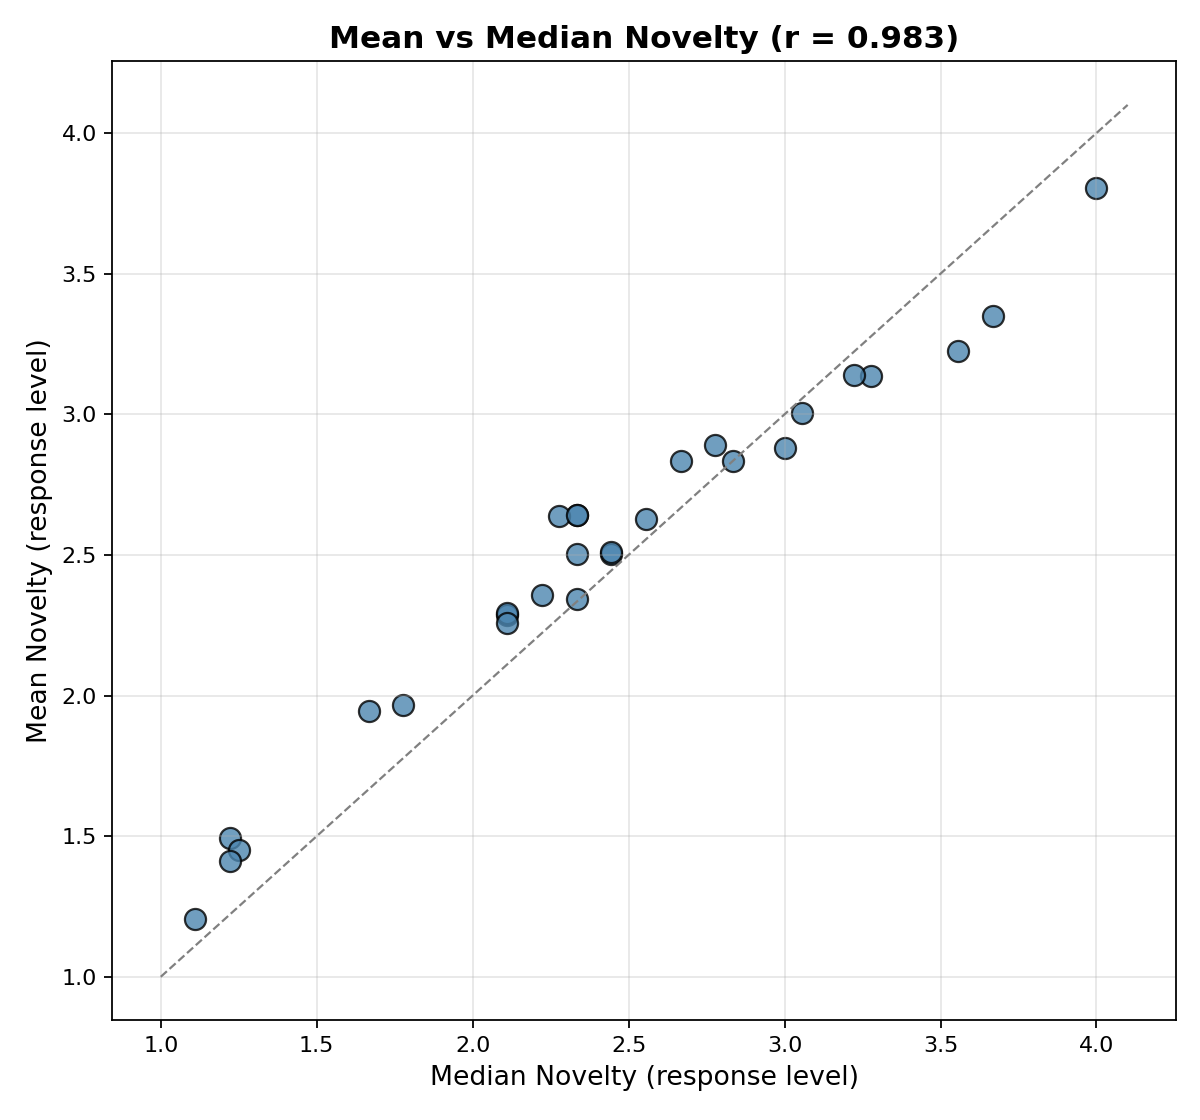
\includegraphics[width=0.7\textwidth]{figures_v2/appendix_mean_vs_median_novelty.png}
\caption{Mean vs. median Novelty scores (response level, 28 model $\times$ condition cells). The high correlation ($r = 0.983$) indicates that results are robust against outliers.}
\label{fig:mean_median_novelty}
\end{figure}

The correlation between mean and median Novelty scores is $r = 0.983$ ($p < 0.001$), confirming that our findings are not artifacts of extreme outliers. Mean-median differences at the response level range from $-0.33$ to $+0.36$ across the 28 cells, reflecting the coarser scale of response-level averages; the near-unity correlation confirms that the rank ordering of cells is preserved.
\newpage
\subsection*{A.2 Complete Descriptive Statistics for Novelty}

Table~\ref{tab:desc_novelty_full} presents the complete response-level descriptive statistics for Novelty across all models and conditions (n = number of responses; each response is the mean of nine judge ratings). GPT Culture\_5 includes 120 responses across the 100 problems (20 problems were generated twice).

\begin{table}[H]
\centering
\caption{Complete Descriptive Statistics for Novelty}
\label{tab:desc_novelty_full}
\begin{tabular}{lcccccc}
\toprule
\multirow{2}{*}{Model} & \multirow{2}{*}{Condition} & \multicolumn{2}{c}{Novelty} & \multirow{2}{*}{n} \\
\cmidrule(lr){3-4}
 & & Mean & SD & \\
\midrule
\multirow{4}{*}{Claude} & Culture\_5 & 3.81 & 0.64 & 100 \\
 & Culture\_Expert & 3.14 & 1.06 & 100 \\
 & Culture\_11 & 2.89 & 0.95 & 100 \\
 & Large Baseline & 2.84 & 1.09 & 100 \\
\midrule
\multirow{4}{*}{DeepSeek} & Culture\_5 & 3.35 & 1.02 & 100 \\
 & Culture\_Expert & 3.14 & 1.03 & 100 \\
 & Culture\_11 & 2.64 & 1.00 & 100 \\
 & Large Baseline & 2.64 & 1.13 & 100 \\
\midrule
\multirow{4}{*}{GPT} & Culture\_5 & 3.22 & 0.99 & 120 \\
 & Culture\_Expert & 3.00 & 1.04 & 100 \\
 & Culture\_11 & 2.88 & 1.02 & 100 \\
 & Large Baseline & 2.64 & 1.06 & 100 \\
\midrule
\multirow{4}{*}{Llama} & Culture\_5 & 2.50 & 0.74 & 100 \\
 & Culture\_Expert & 2.34 & 0.68 & 100 \\
 & Culture\_11 & 1.97 & 0.68 & 100 \\
 & Large Baseline & 2.29 & 0.86 & 100 \\
\midrule
\multirow{4}{*}{Mistral} & Culture\_5 & 2.50 & 0.74 & 100 \\
 & Culture\_Expert & 2.29 & 0.74 & 100 \\
 & Culture\_11 & 1.95 & 0.80 & 100 \\
 & Large Baseline & 2.36 & 0.85 & 99 \\
\midrule
\multirow{4}{*}{Qwen} & Culture\_5 & 2.63 & 0.71 & 100 \\
 & Culture\_Expert & 2.51 & 0.69 & 100 \\
 & Culture\_11 & 2.26 & 0.72 & 100 \\
 & Large Baseline & 2.83 & 1.05 & 100 \\
\midrule
\multirow{4}{*}{Gemini} & Culture\_5 & 1.49 & 0.73 & 100 \\
 & Culture\_Expert & 1.45 & 0.56 & 100 \\
 & Culture\_11 & 1.21 & 0.34 & 100 \\
 & Large Baseline & 1.41 & 0.55 & 99 \\
\bottomrule
\end{tabular}
\end{table}

\newpage
\subsection*{A.3 Complete Domain-Specific Effect Sizes for Novelty}

Table~\ref{tab:domain_novelty_full} presents the complete domain-specific effect sizes for all persona-domain combinations.

\begin{table}[H]
\centering
\caption{Complete Domain-Specific Effect Sizes for Novelty}
\label{tab:domain_novelty_full}
\begin{tabular}{lcccc}
\toprule
\textbf{Persona} & \textbf{Creative} & \textbf{General Knowledge} & \textbf{Instruction} & \textbf{Reasoning} \\
\midrule
Culture\_5 & 0.233 & 0.628 & 0.185 & 0.545 \\
Culture\_Expert & 0.036 & 0.223 & 0.092 & 0.210 \\
Culture\_11 & -0.196 & -0.154 & -0.229 & -0.149 \\
\bottomrule
\end{tabular}
\caption*{\footnotesize Positive values indicate improvement over baseline; negative values indicate degradation.}
\end{table}

\newpage
\subsection*{A.4 Power Analysis Details}

Table~\ref{tab:power_novelty_full} presents the post-hoc power analysis results for each model-persona combination.

\begin{table}[H]
\centering
\caption{Post-hoc Power Analysis for Novelty by Model and Persona}
\label{tab:power_novelty_full}
\begin{tabular}{lccc}
\toprule
Model & Culture\_5 & Culture\_Expert & Culture\_11 \\
\midrule
Claude & 1.00 & 0.51 & 0.07 \\
DeepSeek & 1.00 & 0.90 & 0.05 \\
GPT & 0.99 & 0.68 & 0.37 \\
Llama & 0.48 & 0.08 & 0.83 \\
Mistral & 0.26 & 0.08 & 0.94 \\
Qwen & 0.36 & 0.73 & 0.99 \\
Gemini & 0.15 & 0.08 & 0.88 \\
\bottomrule
\end{tabular}
\caption*{\footnotesize Values $>0.80$ indicate sufficient power. Response-level power (n $\approx$ 100 per cell): mean power = 0.544; 38.1\% of comparisons achieved sufficient power.}
\end{table}

\newpage
\subsection*{A.5 Leave-One-Out Sensitivity Results}

Leave-one-out sensitivity analysis confirmed that results are highly stable. Table~\ref{tab:loo_novelty} presents the mean absolute change in effect size when each model was removed.

\begin{table}[H]
\centering
\caption{Leave-One-Out Sensitivity Analysis for Novelty}
\label{tab:loo_novelty}
\begin{tabular}{lc}
\toprule
Removed Model & Mean $|\Delta|$ in Effect Size \\
\midrule
Qwen & 0.083 \\
Claude & 0.065 \\
GPT & 0.050 \\
DeepSeek & 0.049 \\
Mistral & 0.036 \\
Gemini & 0.027 \\
Llama & 0.018 \\
\bottomrule
\end{tabular}
\caption*{\footnotesize Mean absolute change in Cohen's d when each model is removed (response level, 21 effect sizes). 19 of 21 changes satisfy $|\Delta| < 0.1$; the largest is 0.117 (removing Claude, Culture\_5). Qwen and Claude have the largest impact, while Llama has the smallest. No single model drives the observed patterns.}
\end{table}

\newpage
\subsection*{A.6 Model Costs Summary}

Table~\ref{tab:costs_full} summarizes the output token costs per 1M tokens for all models used in the economic analysis.

\begin{table}[H]
\centering
\caption{Model Costs Summary (Output Token Cost per 1M Tokens)}
\label{tab:costs_full}
\begin{tabular}{lccc}
\toprule
Model & Small Model & Large Model & Cost Ratio (Small/Large) \\
\midrule
Claude & \$15.00 (Sonnet) & \$25.00 (Opus) & 0.60 \\
DeepSeek & \$0.42 (Chat) & \$0.42 (Reasoner) & 1.00 \\
GPT & \$2.00 (Mini) & \$15.00 (5.4) & 0.13 \\
Llama & \$0.20 (8B) & \$0.88 (70B) & 0.23 \\
Mistral & \$0.60 (Mixtral) & \$0.30 (Small) & 2.00 \\
Qwen & \$0.30 (7B) & \$1.50 (80B) & 0.20 \\
Gemini & \$1.50 (Flash Lite) & \$12.00 (Pro) & 0.13 \\
\bottomrule
\end{tabular}
\caption*{\footnotesize Note: For Mistral, the "small" model (Mixtral) is actually older and more expensive than the "large" model (Mistral-Small), reflecting our architectural comparison design.}
\end{table}

\newpage
\subsection*{A.7 Results for Other Dimensions (Exploratory)}

Table~\ref{tab:other_dimensions} presents the response-level mean scores for Usefulness, Flexibility, Elaboration, and Cultural Sensitivity. These results are reported as exploratory due to limited inter-rater reliability (Section 3.6).

\begin{table}[H]
\centering
\caption{Mean Scores for Other Dimensions (Exploratory)}
\label{tab:other_dimensions}
\begin{tabular}{lcccccc}
\toprule
Model & Condition & Usefulness & Flexibility & Elaboration & Cultural Sensitivity \\
\midrule
\multirow{4}{*}{Claude} & Culture\_5 & 4.55 & 3.89 & 4.66 & 4.47 \\
 & Culture\_Expert & 4.75 & 3.69 & 4.74 & 4.42 \\
 & Culture\_11 & 4.63 & 3.50 & 4.68 & 4.42 \\
 & Large Baseline & 4.65 & 3.39 & 4.67 & 4.45 \\
\midrule
\multirow{4}{*}{DeepSeek} & Culture\_5 & 4.45 & 3.72 & 4.42 & 4.37 \\
 & Culture\_Expert & 4.70 & 3.67 & 4.83 & 4.42 \\
 & Culture\_11 & 4.47 & 3.30 & 4.45 & 4.31 \\
 & Large Baseline & 4.42 & 3.17 & 4.23 & 4.33 \\
\midrule
\multirow{4}{*}{GPT} & Culture\_5 & 4.71 & 3.63 & 4.41 & 4.49 \\
 & Culture\_Expert & 4.81 & 3.71 & 4.62 & 4.41 \\
 & Culture\_11 & 4.74 & 3.66 & 4.51 & 4.45 \\
 & Large Baseline & 4.71 & 3.27 & 4.50 & 4.55 \\
\midrule
\multirow{4}{*}{Llama} & Culture\_5 & 3.69 & 2.77 & 3.83 & 4.26 \\
 & Culture\_Expert & 4.16 & 2.96 & 4.20 & 4.29 \\
 & Culture\_11 & 3.71 & 2.50 & 3.82 & 3.46 \\
 & Large Baseline & 4.38 & 2.82 & 4.24 & 4.44 \\
\midrule
\multirow{4}{*}{Mistral} & Culture\_5 & 3.70 & 2.84 & 3.81 & 3.88 \\
 & Culture\_Expert & 4.15 & 2.85 & 4.14 & 4.35 \\
 & Culture\_11 & 3.40 & 2.37 & 3.62 & 3.46 \\
 & Large Baseline & 4.54 & 2.97 & 4.38 & 4.50 \\
\midrule
\multirow{4}{*}{Qwen} & Culture\_5 & 4.14 & 3.12 & 4.01 & 4.22 \\
 & Culture\_Expert & 4.42 & 3.19 & 4.38 & 4.47 \\
 & Culture\_11 & 4.30 & 2.82 & 4.15 & 3.65 \\
 & Large Baseline & 4.60 & 3.37 & 4.60 & 4.49 \\
\midrule
\multirow{4}{*}{Gemini} & Culture\_5 & 1.42 & 1.53 & 3.14 & 3.77 \\
 & Culture\_Expert & 1.82 & 1.62 & 3.89 & 3.79 \\
 & Culture\_11 & 1.32 & 1.25 & 3.01 & 3.66 \\
 & Large Baseline & 1.83 & 1.57 & 3.67 & 3.97 \\
\bottomrule
\end{tabular}
\caption*{\footnotesize These results should be interpreted with caution due to limited inter-rater reliability (Fleiss' $\kappa$: Usefulness $= 0.32$, Flexibility $= 0.32$, Elaboration $= 0.31$, Cultural Sensitivity $= 0.17$). Values are response-level means (n $\approx$ 100 per cell).}
\end{table}

\newpage
\subsection*{A.8 Pure Persona Effects (Small Baseline vs. Small+Persona)}

This supplementary analysis isolates the pure effect of each persona by comparing 
small models with personas against their own small model baseline (no persona). 
While our main analysis (Section 4) addresses the economic question of whether 
small+persona can match large model performance at lower cost, this analysis 
answers a different question: \textit{does adding a persona improve the small 
model over its own baseline?}

Positive Cohen's \(d\) values indicate that the persona improved Novelty relative 
to the small baseline. Negative values indicate the persona harmed performance. 
All comparisons use Novelty scores (the primary dimension; full-data inter-rater 
reliability is fair, \(\kappa = 0.33\)). Statistical significance is determined using 
FDR-corrected \(p < 0.05\) (indicated by \(^*\)).

\begin{table}[H]
\centering
\caption{Pure Persona Effects (Small Baseline vs. Small+Persona) for Novelty}
\label{tab:pure_persona}
\begin{tabular}{llccc}
\toprule
Model & Persona & Baseline Mean & Persona Mean & Cohen's d \\
\midrule
Claude & Culture 5 & 2.82 & 3.81 & 1.101$^*$ \\
Claude & Culture Expert & 2.82 & 3.14 & 0.296 \\
Claude & Culture 11 & 2.82 & 2.89 & 0.073 \\
DeepSeek & Culture 5 & 2.91 & 3.35 & 0.432$^*$ \\
DeepSeek & Culture Expert & 2.91 & 3.14 & 0.224 \\
DeepSeek & Culture 11 & 2.91 & 2.64 & -0.258 \\
GPT & Culture 5 & 2.76 & 3.22 & 0.448$^*$ \\
GPT & Culture Expert & 2.76 & 3.00 & 0.228 \\
GPT & Culture 11 & 2.76 & 2.88 & 0.115 \\
Llama & Culture 5 & 2.22 & 2.50 & 0.386$^*$ \\
Llama & Culture Expert & 2.22 & 2.34 & 0.173 \\
Llama & Culture 11 & 2.22 & 1.97 & -0.374$^*$ \\
Qwen & Culture 5 & 2.35 & 2.63 & 0.379$^*$ \\
Qwen & Culture Expert & 2.35 & 2.51 & 0.221 \\
Qwen & Culture 11 & 2.35 & 2.26 & -0.120 \\
Mistral & Culture 5 & 2.24 & 2.50 & 0.345$^*$ \\
Mistral & Culture Expert & 2.24 & 2.29 & 0.075 \\
Mistral & Culture 11 & 2.24 & 1.95 & -0.363$^*$ \\
Gemini & Culture 5 & 1.41 & 1.49 & 0.130 \\
Gemini & Culture Expert & 1.41 & 1.45 & 0.077 \\
Gemini & Culture 11 & 1.41 & 1.21 & -0.396$^*$ \\
\bottomrule
\end{tabular}
\caption*{\footnotesize $^*$p < 0.05 (FDR-corrected). Positive Cohen's d indicates improvement from persona. Baseline = small model with no persona. Persona = small model with persona.}
\end{table}

The pure persona effects are consistent with our main findings: 
Culture\_5 improves Novelty significantly for five of seven models (largest 
effect: Claude, \(d = 1.101\)), while Culture\_11 shows negative or negligible 
effects for all models. Note that the pure effects are not uniformly larger than 
the main-analysis contrasts: DeepSeek and GPT small baselines outscore their own 
large baselines, so their pure effects (0.432, 0.448) are smaller than the 
large-baseline contrasts (0.664, 0.570).


\printbibliography
\end{document}